%% ============================================================
%% Analisis Indeks Iklim Ekstrem ETCCDI di Kabupaten Kebumen
%% Berbasis Data ERA5-Land dan Multi-Satelit (2000-2025)
%% ============================================================
%% Kompilasi: pdflatex main.tex (2x untuk referensi silang)
%% ============================================================

\documentclass[12pt, a4paper]{article}

\usepackage[T1]{fontenc}
\usepackage[utf8]{inputenc}
\usepackage{lmodern}
\usepackage{microtype}
\usepackage[indonesian]{babel}
\usepackage[top=2.5cm, bottom=2.5cm, left=3.0cm, right=2.5cm, headheight=15pt]{geometry}
\usepackage{fancyhdr}
\pagestyle{fancy}
\fancyhf{}
\fancyhead[L]{\small\textit{Analisis Iklim ETCCDI Kebumen (2000--2025)}}
\fancyhead[R]{\small\thepage}
\renewcommand{\headrulewidth}{0.4pt}
\usepackage{amsmath, amssymb}
\usepackage{graphicx}
\usepackage{float}
\usepackage[labelfont=bf, font=small, justification=centering]{caption}
\usepackage{subcaption}
\graphicspath{{figures/}}
\usepackage{booktabs}
\usepackage{multirow}
\usepackage{longtable}
\usepackage{array}
\usepackage{tabularx}
\usepackage{colortbl}
\usepackage[table]{xcolor}

\definecolor{headerblue}{RGB}{31, 78, 121}
\definecolor{rowgray}{RGB}{242, 242, 242}
\definecolor{signred}{RGB}{197, 27, 27}
\definecolor{signgreen}{RGB}{26, 120, 49}

\usepackage[colorlinks=true, linkcolor=headerblue, citecolor=headerblue, urlcolor=headerblue,
  pdftitle={Analisis Iklim ETCCDI Kebumen 2000-2025},
  pdfauthor={Evan Alif Widhyatma}]{hyperref}

\usepackage[numbers, sort&compress]{natbib}
\bibliographystyle{apalike}
\usepackage{enumitem}
\usepackage{setspace}
\usepackage{parskip}
\setlength{\parindent}{0pt}
\setlength{\parskip}{6pt}

\newcommand{\degC}{$^{\circ}$C}
\newcommand{\etccdi}{\textsc{etccdi}}
\newcommand{\era}{\textsc{era5-land}}
\newcommand{\mk}{\textit{Mann-Kendall}}
\newcommand{\sens}{\textit{Sen's Slope}}

\begin{document}

%% HALAMAN JUDUL
\begin{titlepage}
  \centering
  \vspace*{1.5cm}
  {\Large\bfseries\color{headerblue}
    Analisis Indeks Iklim Ekstrem {ETCCDI}\\[0.4em]
    di Kabupaten Kebumen, Jawa Tengah\\[0.4em]
    Berbasis Data {ERA5-Land} dan Satelit\\
    (2000--2025)
  }
  \vspace{1.5cm}
  \vspace{0.8cm}

  {\large
    \textbf{Evan Alif Widhyatma}\\[0.3em]
    \textit{Program Studi Sains Data}\\[0.2em]
    \textit{Universitas Putra Bangsa}\\[0.2em]
    \texttt{evanalifwidhyatma@gmail.com}
  }
\end{titlepage}

\tableofcontents
\listoffigures
\listoftables
\newpage

%% ABSTRAK
\section*{Abstrak}
\addcontentsline{toc}{section}{Abstrak}

Penelitian ini menganalisis 27 indeks iklim ekstrem inti yang ditetapkan oleh \textit{Expert Team on Climate Change Detection and Indices} (\textsc{etccdi}) di Kabupaten Kebumen, Jawa Tengah, selama periode 26 tahun (2000--2025). Data suhu dan curah hujan harian diperoleh dari reanalisis \textsc{era5-land} (ECMWF), dilengkapi dengan empat produk presipitasi satelit: CHIRPS\_RNL, GSMaP, IMERG, dan ERA5-Land. Uji tren non-parametrik \textit{Mann-Kendall} dan estimasi kemiringan \textit{Sen's Slope} diterapkan untuk setiap indeks menggunakan periode baseline WMO 2001--2020.

Hasil menunjukkan peningkatan nyata pada indeks suhu malam hari, terutama \textbf{TN90p} (Malam Hangat) yang meningkat signifikan dengan $Z_{MK} = 4{,}30$ ($p < 0{,}001$) dan laju $+7{,}17\%$ per dekade, serta \textbf{TNx} (Suhu Minimum Tertinggi) dengan laju $+0{,}37$\degC{} per dekade. Sebaliknya, indeks dingin \textbf{TN10p} menurun dengan laju $-4{,}78\%$ per dekade, mengindikasikan \textit{warming asymmetry} yang lebih kuat pada suhu minimum dibandingkan suhu maksimum. Pada indeks presipitasi, \textbf{CWD} (Hari Basah Berturut-turut) menunjukkan penurunan signifikan ($Z_{MK} = -2{,}29$, $p = 0{,}022$) sebesar $-10{,}77$ hari per dekade.

\textbf{Kata kunci:} ETCCDI; indeks iklim ekstrem; ERA5-Land; Kabupaten Kebumen; Mann-Kendall; tren iklim; curah hujan ekstrem; suhu ekstrem.

\newpage

%% 1. PENDAHULUAN
\section{Pendahuluan}

\subsection{Latar Belakang}

Perubahan iklim global telah meningkatkan frekuensi dan intensitas kejadian cuaca ekstrem di berbagai belahan dunia, termasuk Indonesia \citep{ipcc2021}. Kabupaten Kebumen, yang terletak di pesisir selatan Jawa Tengah ($7{,}28^{\circ}$--$7{,}80^{\circ}$LS; $109{,}22^{\circ}$--$109{,}83^{\circ}$BT), merupakan kawasan rentan dengan karakteristik iklim monsun tropis yang kompleks. Variabilitas curah hujan yang tinggi, banjir tahunan di Sungai Luk Ulo, dan potensi kekeringan pada musim kemarau menjadikan kabupaten ini sebagai studi kasus yang relevan untuk analisis iklim ekstrem.

Standarisasi pengukuran indeks iklim ekstrem oleh \etccdi{} menyediakan kerangka kerja ilmiah yang komprehensif untuk mendeteksi dan memantau perubahan iklim \citep{alexander2006,zhang2011}. Kumpulan 27 indeks inti \etccdi{} mencakup 16 indeks suhu dan 11 indeks presipitasi yang telah digunakan secara luas dalam kajian iklim regional di seluruh dunia \citep{donat2013}.

\subsection{Rumusan Masalah}

Penelitian ini menjawab pertanyaan-pertanyaan berikut:
\begin{enumerate}
  \item Bagaimana tren jangka panjang 27 indeks \etccdi{} suhu dan presipitasi di Kabupaten Kebumen selama 2000--2025?
  \item Indeks mana yang menunjukkan perubahan statistik yang signifikan berdasarkan uji \mk{}?
  \item Bagaimana perbandingan indeks presipitasi ekstrem antar-produk satelit?
\end{enumerate}

\subsection{Tujuan Penelitian}

\begin{enumerate}
  \item Menghitung 27 indeks \etccdi{} secara tahunan dari data \era{} untuk periode 2000--2025.
  \item Menganalisis tren temporal menggunakan uji \mk{} dan \sens{} dengan tingkat signifikansi $\alpha = 0{,}05$.
  \item Membandingkan indeks presipitasi dari empat produk satelit dalam konteks akurasi regional.
\end{enumerate}

\subsection{Manfaat Penelitian}

Hasil penelitian ini diharapkan menjadi referensi ilmiah untuk perencanaan adaptasi perubahan iklim di Kabupaten Kebumen dan mendukung \textit{Early Warning System} cuaca ekstrem di wilayah ini.

%% 2. TINJAUAN PUSTAKA
\section{Tinjauan Pustaka}

\subsection{Indeks Iklim Ekstrem ETCCDI}

\etccdi{} (\textit{Expert Team on Climate Change Detection and Indices}) adalah kelompok pakar yang dibentuk oleh \textit{World Meteorological Organization} (WMO) dan \textit{World Climate Research Programme} (WCRP) untuk mengembangkan dan menstandardisasi definisi indeks iklim ekstrem \citep{zhang2011}. Dua puluh tujuh indeks inti yang ditetapkan dibagi menjadi dua kategori:

\begin{itemize}
  \item \textbf{Indeks Suhu (16 indeks):} Nilai absolut (TXx, TXn, TNx, TNn), berbasis ambang batas (SU, TR, FD, ID), berbasis persentil (TX10p, TX90p, TN10p, TN90p), durasi gelombang panas/dingin (WSDI, CSDI), rentang suhu harian (DTR), dan panjang musim tanam (GSL).
  \item \textbf{Indeks Presipitasi (11 indeks):} Presipitasi ekstrem absolut (Rx1day, Rx5day), intensitas (SDII), total (PRCPTOT), ambang batas (R10mm, R20mm, R$nn$mm), berbasis persentil (R95pTOT, R99pTOT), dan hari kering/basah (CDD, CWD).
\end{itemize}

\subsection{Data ERA5-Land}

ERA5-Land merupakan reanalisis atmosfer global beresolusi tinggi dari \textit{European Centre for Medium-Range Weather Forecasts} (ECMWF) dengan resolusi spasial $0{,}1^{\circ}$ ($\sim$9 km) dan resolusi temporal 1 jam. Dataset ini dioptimalkan untuk variabel permukaan tanah dan dokumentasi resminya menunjukkan peningkatan representasi hidrologi dibandingkan ERA5 \citep{munoz2021}.

\subsection{Uji Mann-Kendall dan Sen's Slope}

Uji \mk{} adalah uji non-parametrik yang cocok untuk mendeteksi tren monotonik dalam deret waktu hidroklimatologi karena tidak memerlukan asumsi distribusi normal \citep{mann1945,kendall1975}. Statistik $Z$ digunakan untuk menguji hipotesis nol tidak adanya tren. \sens{} memberikan estimasi kemiringan tren median yang robust terhadap \textit{outlier} \citep{sen1968}.

\subsection{Iklim Kebumen}

Kabupaten Kebumen beriklim tropis dengan tipe iklim Am--Aw menurut klasifikasi K\"{o}ppen, dengan curah hujan tahunan rata-rata 2.000--3.500 mm dan musim hujan Oktober--April. Suhu udara relatif stabil sepanjang tahun dengan rata-rata 25--28\degC{} di dataran rendah. Fenomena El Ni\~{n}o Southern Oscillation (ENSO) mempengaruhi variabilitas curah hujan secara signifikan.

%% 3. METODOLOGI
\section{Metodologi}

\subsection{Wilayah dan Periode Studi}

Wilayah studi mencakup Kabupaten Kebumen dengan fokus pada koordinat Stasiun AWS Jerukagung, Kecamatan Klirong ($-7{,}68^{\circ}$LS; $109{,}50^{\circ}$BT, elevasi $\pm$12 m dpl). Periode analisis meliputi 26 tahun kalender penuh: 1 Januari 2000 hingga 31 Desember 2025 (9.497 hari, 6 tahun kabisat: 2000, 2004, 2008, 2012, 2016, 2020, 2024).

\subsection{Sumber Data}

\subsubsection{ERA5-Land (Data Primer Suhu dan Presipitasi)}

Data \era{} diunduh melalui \textit{Google Earth Engine} (GEE) menggunakan koleksi \texttt{ECMWF/ERA5\_LAND/HOURLY\_AGGR}. Variabel yang digunakan:
\begin{itemize}
  \item \texttt{temperature\_2m}: suhu udara pada ketinggian 2 m (K $\to$ \degC{})
  \item \texttt{total\_precipitation\_hourly}: total presipitasi per jam (m $\to$ mm)
\end{itemize}
Data diagregasi menjadi nilai harian (TX, TN, PR) dalam Waktu Indonesia Barat (WIB = UTC+7).

\subsubsection{Produk Presipitasi Satelit (Komparasi)}

Empat produk satelit digunakan:
\begin{itemize}
  \item \textbf{CHIRPS\_RNL}: Climate Hazards Group InfraRed Precipitation, resolusi $0{,}05^{\circ}$, harian
  \item \textbf{GSMaP}: Global Satellite Mapping of Precipitation, resolusi $0{,}1^{\circ}$
  \item \textbf{IMERG}: Integrated Multi-satellitE Retrievals for GPM, resolusi $0{,}1^{\circ}$
  \item \textbf{ERA5-Land}: Digunakan sebagai referensi utama
\end{itemize}

\subsection{Agregasi Data Harian}

Dari data jam-an ERA5-Land, agregasi harian dilakukan:
\begin{align}
  TX_d &= \max_{h \in d}\{T_{2m,h}\} \\
  TN_d &= \min_{h \in d}\{T_{2m,h}\} \\
  PR_d &= \sum_{h \in d} P_h
\end{align}
di mana $T_{2m,h}$ adalah suhu 2 m pada jam ke-$h$ dalam hari $d$, dan $P_h$ adalah presipitasi jam-an.

\subsection{Perhitungan 27 Indeks ETCCDI}

\subsubsection{Baseline Period dan Persentil}

Periode baseline 2001--2020 (standar WMO) digunakan untuk menghitung persentil kalender harian dengan jendela geser 5 hari. Untuk setiap hari kalender $d_0 \in \{1, \ldots, 366\}$:
\begin{equation}
  \Theta^{TX}_{p,d_0} = \text{percentile}_p\bigl(\{TX_{d} : d \in \mathcal{W}_{d_0}^{5}, \text{year} \in [2001, 2020]\}\bigr)
\end{equation}

Untuk presipitasi, persentil $p_{95}$ dan $p_{99}$ dihitung dari distribusi curah hujan hari-hari basah ($PR \geq 1{,}0$ mm) selama baseline.

\subsubsection{Definisi Matematis Indeks Suhu (16 Indeks)}

\begin{longtable}[l]{@{}p{1.4cm}p{4.5cm}p{7.5cm}@{}}
  \caption{Definisi matematis 16 Indeks Suhu ETCCDI}\label{tab:def_temp}\\
  \toprule
  \textbf{Kode} & \textbf{Nama} & \textbf{Formula / Definisi} \\
  \midrule
  \endfirsthead
  \multicolumn{3}{c}{\footnotesize(lanjutan Tabel~\ref{tab:def_temp})}\\
  \toprule
  \textbf{Kode} & \textbf{Nama} & \textbf{Formula / Definisi} \\
  \midrule
  \endhead
  \bottomrule
  \endfoot
  TXx  & Suhu Maks.\ Tertinggi & $\text{TXx}_y = \max_{d \in y}\{TX_d\}$ \\[3pt]
  TXn  & Suhu Maks.\ Terendah  & $\text{TXn}_y = \min_{d \in y}\{TX_d\}$ \\[3pt]
  TNx  & Suhu Min.\ Tertinggi  & $\text{TNx}_y = \max_{d \in y}\{TN_d\}$ \\[3pt]
  TNn  & Suhu Min.\ Terendah   & $\text{TNn}_y = \min_{d \in y}\{TN_d\}$ \\[3pt]
  SU   & \textit{Summer Days}  & $\text{SU}_y = \#\{d \in y : TX_d > 25\text{\degC}\}$ \\[3pt]
  TR   & \textit{Tropical Nights} & $\text{TR}_y = \#\{d \in y : TN_d > 20\text{\degC}\}$ \\[3pt]
  FD   & \textit{Frost Days}   & $\text{FD}_y = \#\{d \in y : TN_d < 0\text{\degC}\}$ \\[3pt]
  ID   & \textit{Ice Days}     & $\text{ID}_y = \#\{d \in y : TX_d < 0\text{\degC}\}$ \\[3pt]
  TX10p & \textit{Cool Days}   & $\text{TX10p}_y = \frac{100}{N_y}\#\{d \in y : TX_d < \Theta^{TX}_{10,d}\}$ \\[3pt]
  TX90p & \textit{Warm Days}   & $\text{TX90p}_y = \frac{100}{N_y}\#\{d \in y : TX_d > \Theta^{TX}_{90,d}\}$ \\[3pt]
  TN10p & \textit{Cool Nights} & $\text{TN10p}_y = \frac{100}{N_y}\#\{d \in y : TN_d < \Theta^{TN}_{10,d}\}$ \\[3pt]
  TN90p & \textit{Warm Nights} & $\text{TN90p}_y = \frac{100}{N_y}\#\{d \in y : TN_d > \Theta^{TN}_{90,d}\}$ \\[3pt]
  WSDI & \textit{Warm Spell Duration} & Jumlah hari dalam rentang $\geq 6$ hari berurutan dengan $TX_d > \Theta^{TX}_{90,d}$ \\[3pt]
  CSDI & \textit{Cold Spell Duration}  & Jumlah hari dalam rentang $\geq 6$ hari berurutan dengan $TN_d < \Theta^{TN}_{10,d}$ \\[3pt]
  DTR  & \textit{Diurnal Temp.\ Range} & $\text{DTR}_y = \frac{1}{N_y}\sum_{d \in y}(TX_d - TN_d)$ \\[3pt]
  GSL  & \textit{Growing Season Length} & Jumlah hari antara awal dan akhir musim berdasarkan rentang suhu rata-rata enam hari berturut-turut \\
\end{longtable}

\subsubsection{Definisi Matematis Indeks Presipitasi (11 Indeks)}

\begin{longtable}[l]{@{}p{1.8cm}p{4.2cm}p{7.4cm}@{}}
  \caption{Definisi matematis 11 Indeks Presipitasi ETCCDI}\label{tab:def_prec}\\
  \toprule
  \textbf{Kode} & \textbf{Nama} & \textbf{Formula / Definisi} \\
  \midrule
  \endfirsthead
  \multicolumn{3}{c}{\footnotesize(lanjutan Tabel~\ref{tab:def_prec})}\\
  \toprule
  \textbf{Kode} & \textbf{Nama} & \textbf{Formula / Definisi} \\
  \midrule
  \endhead
  \bottomrule
  \endfoot
  Rx1day  & CH Maks.\ 1 Hari & $\text{Rx1day}_y = \max_{d \in y}\{PR_d\}$ \\[3pt]
  Rx5day  & CH Maks.\ 5 Hari & $\text{Rx5day}_y = \max_{d \in y}\left\{\sum_{k=0}^{4} PR_{d-k}\right\}$ \\[3pt]
  SDII    & Intensitas Harian & $\text{SDII}_y = \frac{\sum_{d \in y, PR_d \geq 1} PR_d}{\#\{d \in y : PR_d \geq 1\}}$ \\[3pt]
  PRCPTOT & Total CH Hari Basah & $\text{PRCPTOT}_y = \sum_{d \in y, PR_d \geq 1} PR_d$ \\[3pt]
  R10mm   & Hari Hujan Lebat & $\text{R10mm}_y = \#\{d \in y : PR_d \geq 10\}$ \\[3pt]
  R20mm   & Hari Hujan Sangat Lebat & $\text{R20mm}_y = \#\{d \in y : PR_d \geq 20\}$ \\[3pt]
  Rnnmm   & Hari Hujan Ekstrem ($nn=50$ mm) & $\text{Rnnmm}_y = \#\{d \in y : PR_d \geq 50\}$ (ambang batas BMKG) \\[3pt]
  R95pTOT & Total CH Sangat Basah & $\text{R95pTOT}_y = \sum_{d \in y, PR_d > p_{95}} PR_d$ \\[3pt]
  R99pTOT & Total CH Amat Sangat Basah & $\text{R99pTOT}_y = \sum_{d \in y, PR_d > p_{99}} PR_d$ \\[3pt]
  CDD     & Hari Kering Berurutan & $\text{CDD}_y = \max\{\text{panjang rentang } PR_d < 1 \text{ mm}\}$ \\[3pt]
  CWD     & Hari Basah Berurutan  & $\text{CWD}_y = \max\{\text{panjang rentang } PR_d \geq 1 \text{ mm}\}$ \\
\end{longtable}

\subsection{Analisis Tren: Mann-Kendall dan Sen's Slope}

Uji \mk{} menggunakan statistik:
\begin{equation}
  S = \sum_{i=1}^{n-1}\sum_{j=i+1}^{n} \text{sgn}(x_j - x_i)
\end{equation}

Varians dikoreksi terhadap \textit{ties}:
\begin{equation}
  \text{Var}(S) = \frac{n(n-1)(2n+5) - \sum_t t(t-1)(2t+5)}{18}
\end{equation}

Statistik uji normalisasi:
\begin{equation}
  Z_{MK} = \begin{cases}
    (S-1)/\sqrt{\text{Var}(S)}, & S > 0 \\
    0, & S = 0 \\
    (S+1)/\sqrt{\text{Var}(S)}, & S < 0
  \end{cases}
\end{equation}

\sens{} (kemiringan median Theil-Sen):
\begin{equation}
  \beta = \text{median}\left\{\frac{x_j - x_i}{j - i} : j > i\right\}
\end{equation}

Tingkat signifikansi: *** ($p < 0{,}001$), ** ($p < 0{,}01$), * ($p < 0{,}05$), + ($p < 0{,}1$), ns (tidak signifikan).

%% 4. HASIL DAN PEMBAHASAN
\section{Hasil dan Pembahasan}

\subsection{Statistik Deskriptif 27 Indeks ETCCDI (2000--2025)}

Tabel~\ref{tab:etccdi_summary} menyajikan statistik deskriptif lengkap dan hasil uji tren untuk semua 27 indeks \etccdi{}.

\scriptsize
\setlength{\tabcolsep}{3pt}
\begin{longtable}[c]{@{}llrrrrrrr@{}}
  \caption{Statistik deskriptif dan hasil analisis tren Mann-Kendall 27 Indeks ETCCDI Kebumen (2000--2025). Signifikansi: *** $p<0{,}001$; * $p<0{,}05$; + $p<0{,}1$; ns: tidak signifikan.}\label{tab:etccdi_summary}\\
  \toprule
  \textbf{Kode} & \textbf{Satuan} & \textbf{Rerata} & \textbf{Std} & \textbf{Min} & \textbf{Maks} & \textbf{$Z_{MK}$} & \textbf{Sig.} & \textbf{Slope/Dekade} \\
  \midrule
  \endfirsthead
  \multicolumn{9}{c}{\footnotesize(lanjutan Tabel~\ref{tab:etccdi_summary})}\\
  \toprule
  \textbf{Kode} & \textbf{Satuan} & \textbf{Rerata} & \textbf{Std} & \textbf{Min} & \textbf{Maks} & \textbf{$Z_{MK}$} & \textbf{Sig.} & \textbf{Slope/Dekade} \\
  \midrule
  \endhead
  \bottomrule
  \endfoot
  \multicolumn{9}{@{}l}{\cellcolor{headerblue!15}\textbf{I. Indeks Suhu Udara Ekstrem}} \\
  TXx  & \degC    & 31,69 & 0,79  & 30,57 & 33,75 & 1,76  & +   & +0,267 \degC \\
  TXn  & \degC    & 25,37 & 0,55  & 24,42 & 26,52 & 1,10  & ns  & +0,211 \degC \\
  TNx  & \degC    & 24,98 & 0,46  & 24,22 & 25,94 & 3,39  & *** & +0,370 \degC \\
  TNn  & \degC    & 18,46 & 0,95  & 16,35 & 20,88 & 1,19  & ns  & +0,203 \degC \\
  SU   & hari    & 364,96 & 0,77  & 363   & 366   & 0,68  & ns  & 0,000 \\
  TR   & hari    & 353,96 & 7,95  & 337   & 366   & 2,14  & *   & +5,0 hari \\
  FD   & hari    & 0,00  & 0,00  & 0     & 0     & 0,00  & ns  & 0,000 \\
  ID   & hari    & 0,00  & 0,00  & 0     & 0     & 0,00  & ns  & 0,000 \\
  TX10p & \%     & 9,94  & 4,30  & 1,91  & 18,31 & $-$2,25 & * & $-$2,740\% \\
  TX90p & \%     & 12,37 & 10,14 & 1,91  & 46,45 & 3,57  & *** & +6,393\% \\
  TN10p & \%     & 9,06  & 5,14  & 0,55  & 18,36 & $-$3,46 & *** & $-$4,781\% \\
  TN90p & \%     & 13,79 & 15,47 & 1,92  & 64,21 & 4,30  & *** & +7,165\% \\
  WSDI & hari    & 9,08  & 15,87 & 0     & 58    & 1,64  & ns  & 0,000 hari \\
  CSDI & hari    & 1,35  & 3,47  & 0     & 14    & $-$2,19 & * & 0,000 hari \\
  DTR  & \degC   & 5,87  & 0,35  & 5,31  & 6,48  & $-$0,84 & ns & $-$0,073 \degC \\
  GSL  & hari    & 365,27 & 0,45 & 365   & 366   & $-$0,17 & ns & 0,000 \\
  \midrule
  \multicolumn{9}{@{}l}{\cellcolor{signgreen!10}\textbf{II. Indeks Curah Hujan Ekstrem}} \\
  Rx1day  & mm   & 116,03 & 56,96 & 42,48 & 278,96 & 0,84  & ns  & +13,98 mm \\
  Rx5day  & mm   & 222,27 & 76,37 & 110,77 & 380,31 & 0,88  & ns  & +14,59 mm \\
  SDII    & mm/hr & 9,67  & 1,31  & 7,16  & 12,75  & 1,72  & +   & +0,689 mm/hr \\
  PRCPTOT & mm   & 2.734,33 & 608,63 & 1.617,59 & 3.871,13 & 0,53 & ns & +127,82 mm \\
  R10mm   & hari & 92,27 & 20,91 & 49    & 147    & 0,93  & ns  & +5,5 hari \\
  R20mm   & hari & 30,46 & 9,60  & 16    & 49     & 0,77  & ns  & +1,905 hari \\
  Rnnmm   & hari & 3,62  & 2,98  & 0     & 12     & 1,52  & ns  & +1,25 hari \\
  R95pTOT & mm   & 734,59 & 385,08 & 291,64 & 1.718,43 & 1,15 & ns & +146,17 mm \\
  R99pTOT & mm   & 313,99 & 267,70 & 0,00  & 1.095,40 & 1,64 & ns & +120,92 mm \\
  CDD     & hari & 13,04 & 6,84  & 2     & 28     & $-$0,64 & ns & $-$1,25 hari \\
  CWD     & hari & 68,23 & 24,15 & 34    & 128    & $-$2,30 & * & $-$10,77 hari \\
\end{longtable}
\normalsize

\subsection{Indeks Suhu: Tren dan Pola Temporal}

\subsubsection{Suhu Absolut (TXx, TXn, TNx, TNn)}

Gambar~\ref{fig:temp_absolut} menunjukkan tren temporal indeks suhu absolut. Suhu maksimum tertinggi (\textbf{TXx}) rata-rata mencapai 31,69\degC{} dengan tren lemah naik ($Z_{MK} = 1{,}76$, $p = 0{,}078$; laju +0,267\degC{}/dekade). Nilai puncak TXx tertinggi terjadi pada 2023 (33,75\degC{}), terkait dengan El Ni\~{n}o kuat 2023/2024.

\textbf{TNx} (Suhu Minimum Tertinggi) menunjukkan tren naik paling signifikan: $Z_{MK} = 3{,}39$ ($p = 0{,}0007$, ***) dengan laju +0,37\degC{}/dekade. Ini konsisten dengan fenomena \textit{amplified warming at night} di Asia Tenggara.

\begin{figure}[H]
  \centering
  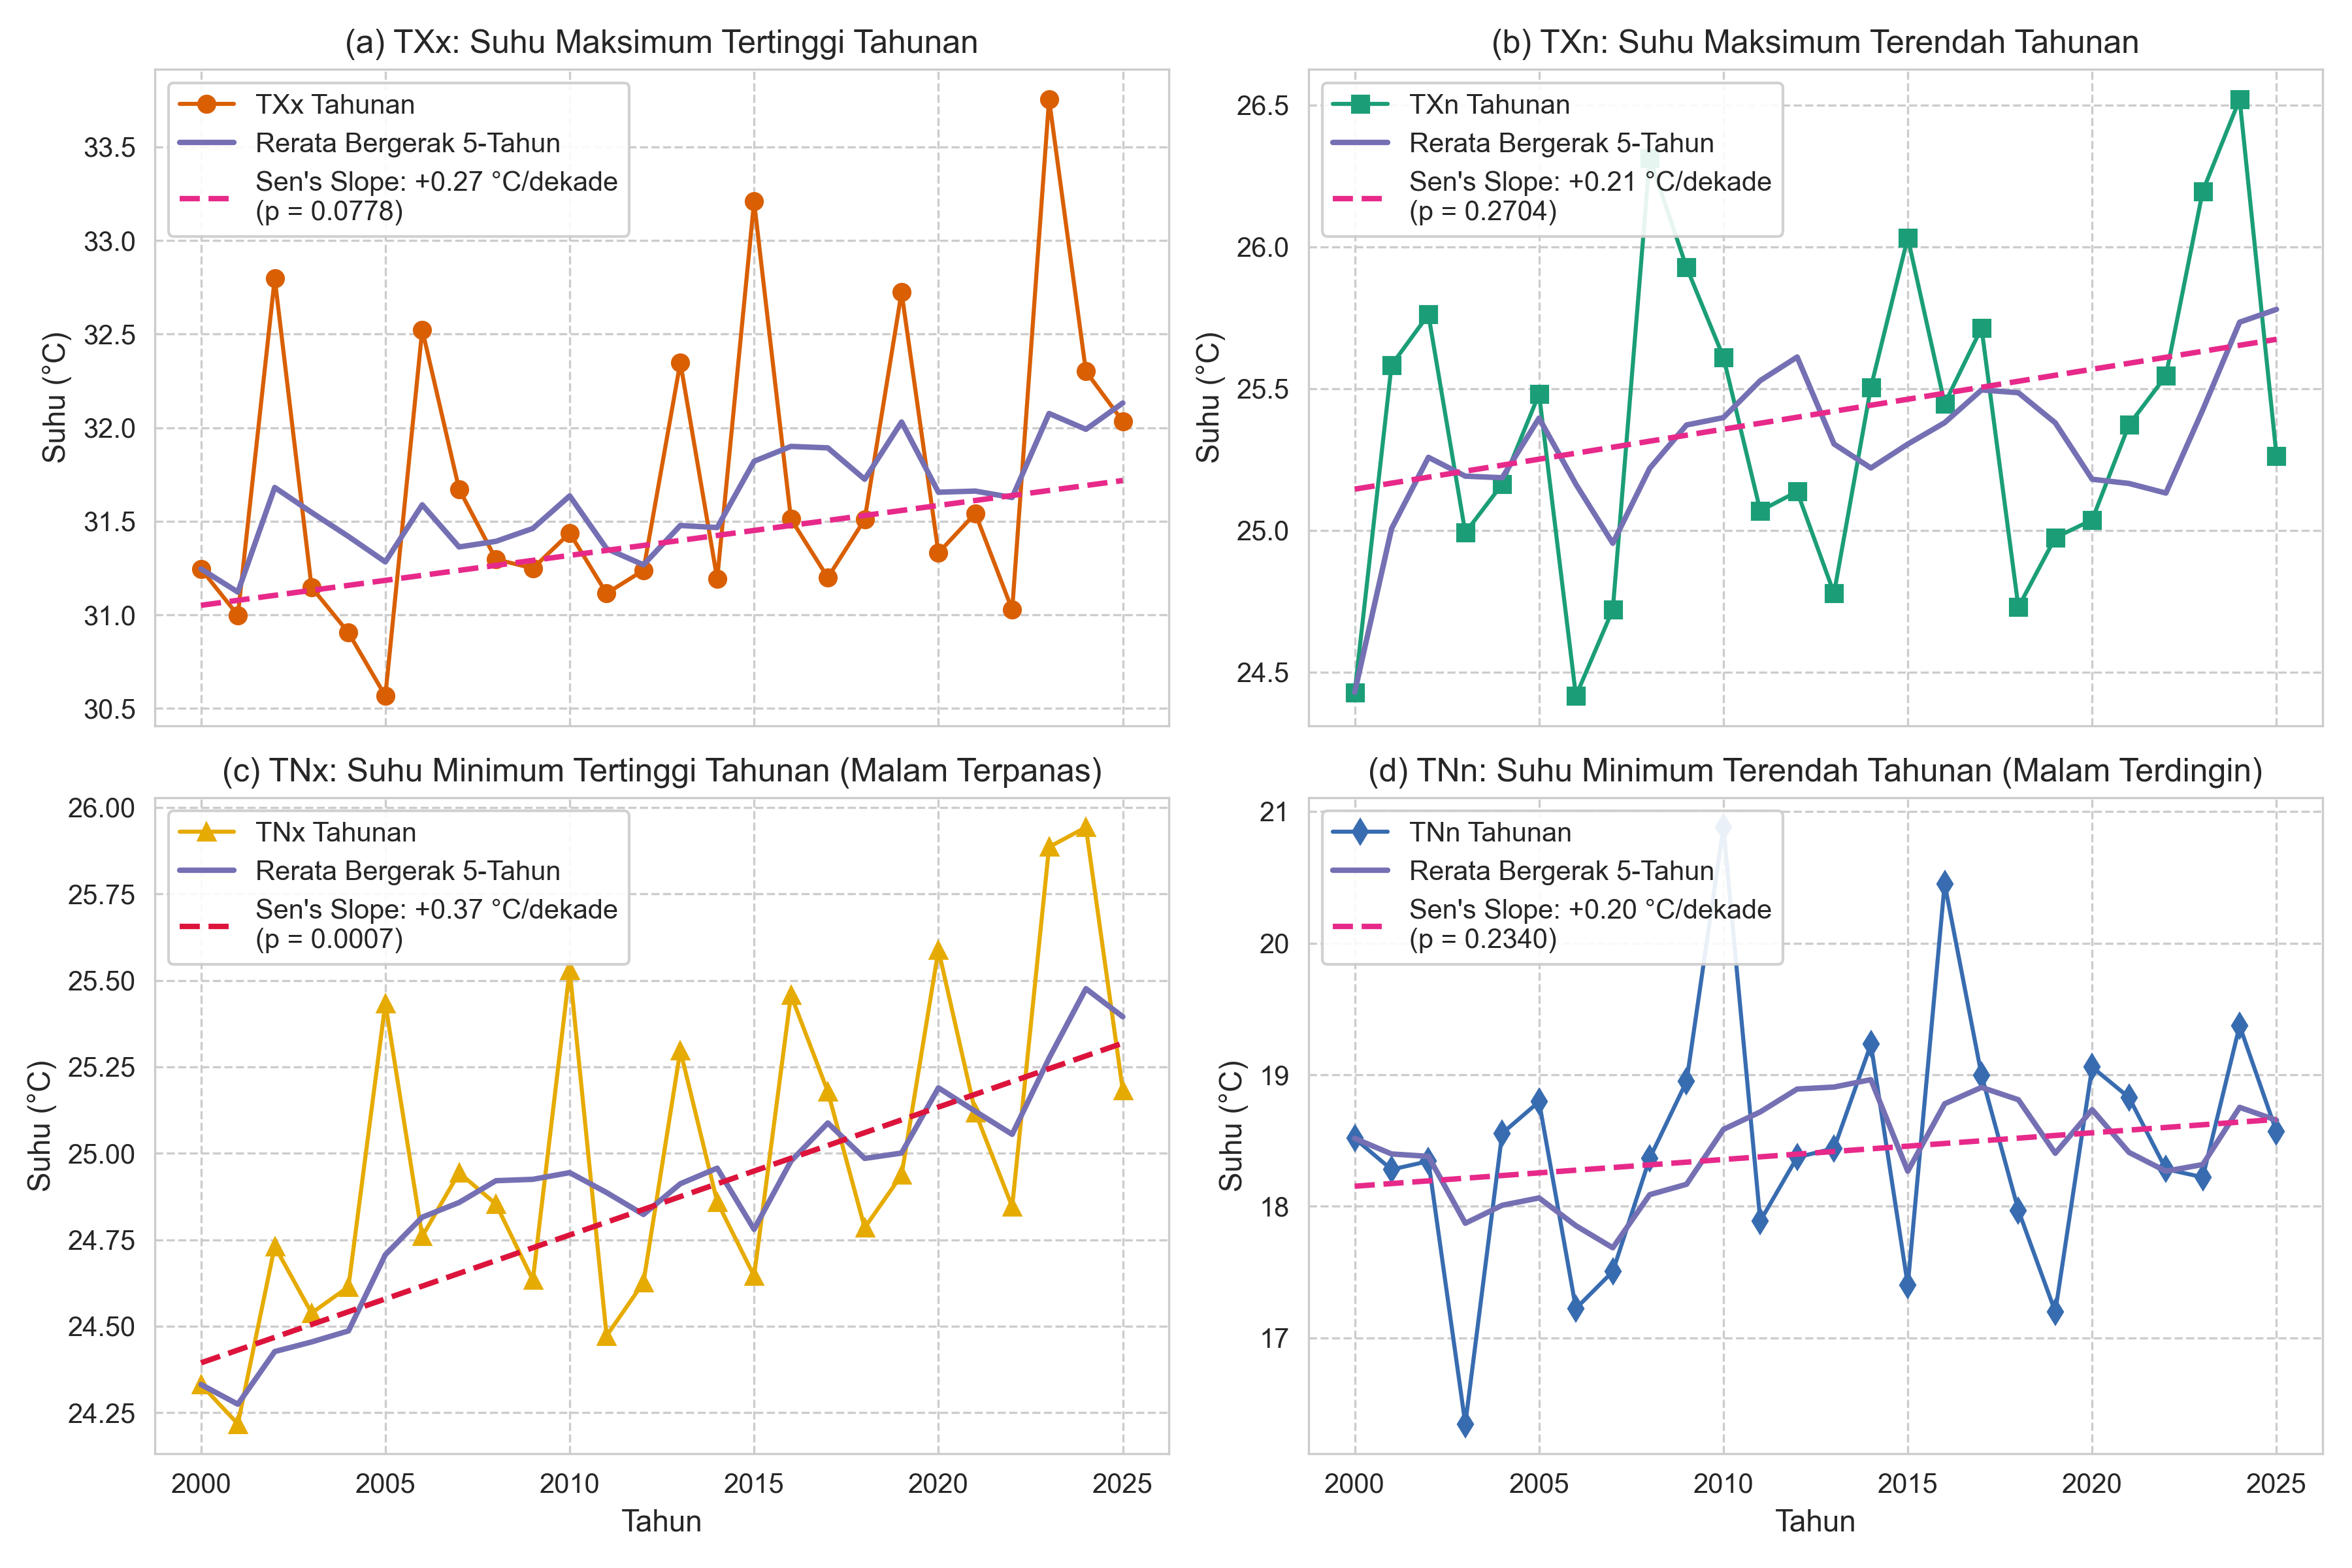
\includegraphics[width=\linewidth]{fig1_temperature_extremes_absolut.png}
  \caption{Tren tahunan indeks suhu absolut TXx, TXn, TNx, dan TNn di Kabupaten Kebumen (2000--2025) berdasarkan ERA5-Land. Garis putus-putus menunjukkan tren linier Sen's Slope.}
  \label{fig:temp_absolut}
\end{figure}

\subsubsection{Indeks Berbasis Persentil (TX10p, TX90p, TN10p, TN90p)}

Gambar~\ref{fig:temp_percentiles} menampilkan evolusi empat indeks persentil suhu. Temuan paling signifikan:

\begin{itemize}
  \item \textbf{TN90p} (Malam Hangat): tren naik paling kuat, $Z_{MK} = 4{,}30$ ($p < 0{,}001$, ***), laju +7,165\%/dekade. Pada 2024, TN90p mencapai 64,2\%---lebih dari separuh malam mengalami suhu di atas persentil ke-90.
  \item \textbf{TX90p} (Siang Panas): tren naik signifikan $Z_{MK} = 3{,}57$ ($p < 0{,}001$, ***), laju +6,393\%/dekade.
  \item \textbf{TN10p} (Malam Dingin): tren turun signifikan $Z_{MK} = -3{,}46$ ($p < 0{,}001$, ***), laju $-$4,781\%/dekade.
  \item \textbf{TX10p} (Siang Dingin): tren turun signifikan $Z_{MK} = -2{,}25$ ($p = 0{,}024$, *), laju $-$2,740\%/dekade.
\end{itemize}

Pola ini mencerminkan \textit{warming asymmetry}: indeks suhu minimum berubah lebih cepat (7,0\% dan 4,6\%/dekade) dibandingkan indeks suhu maksimum (6,3\% dan 2,6\%/dekade).

\begin{figure}[H]
  \centering
  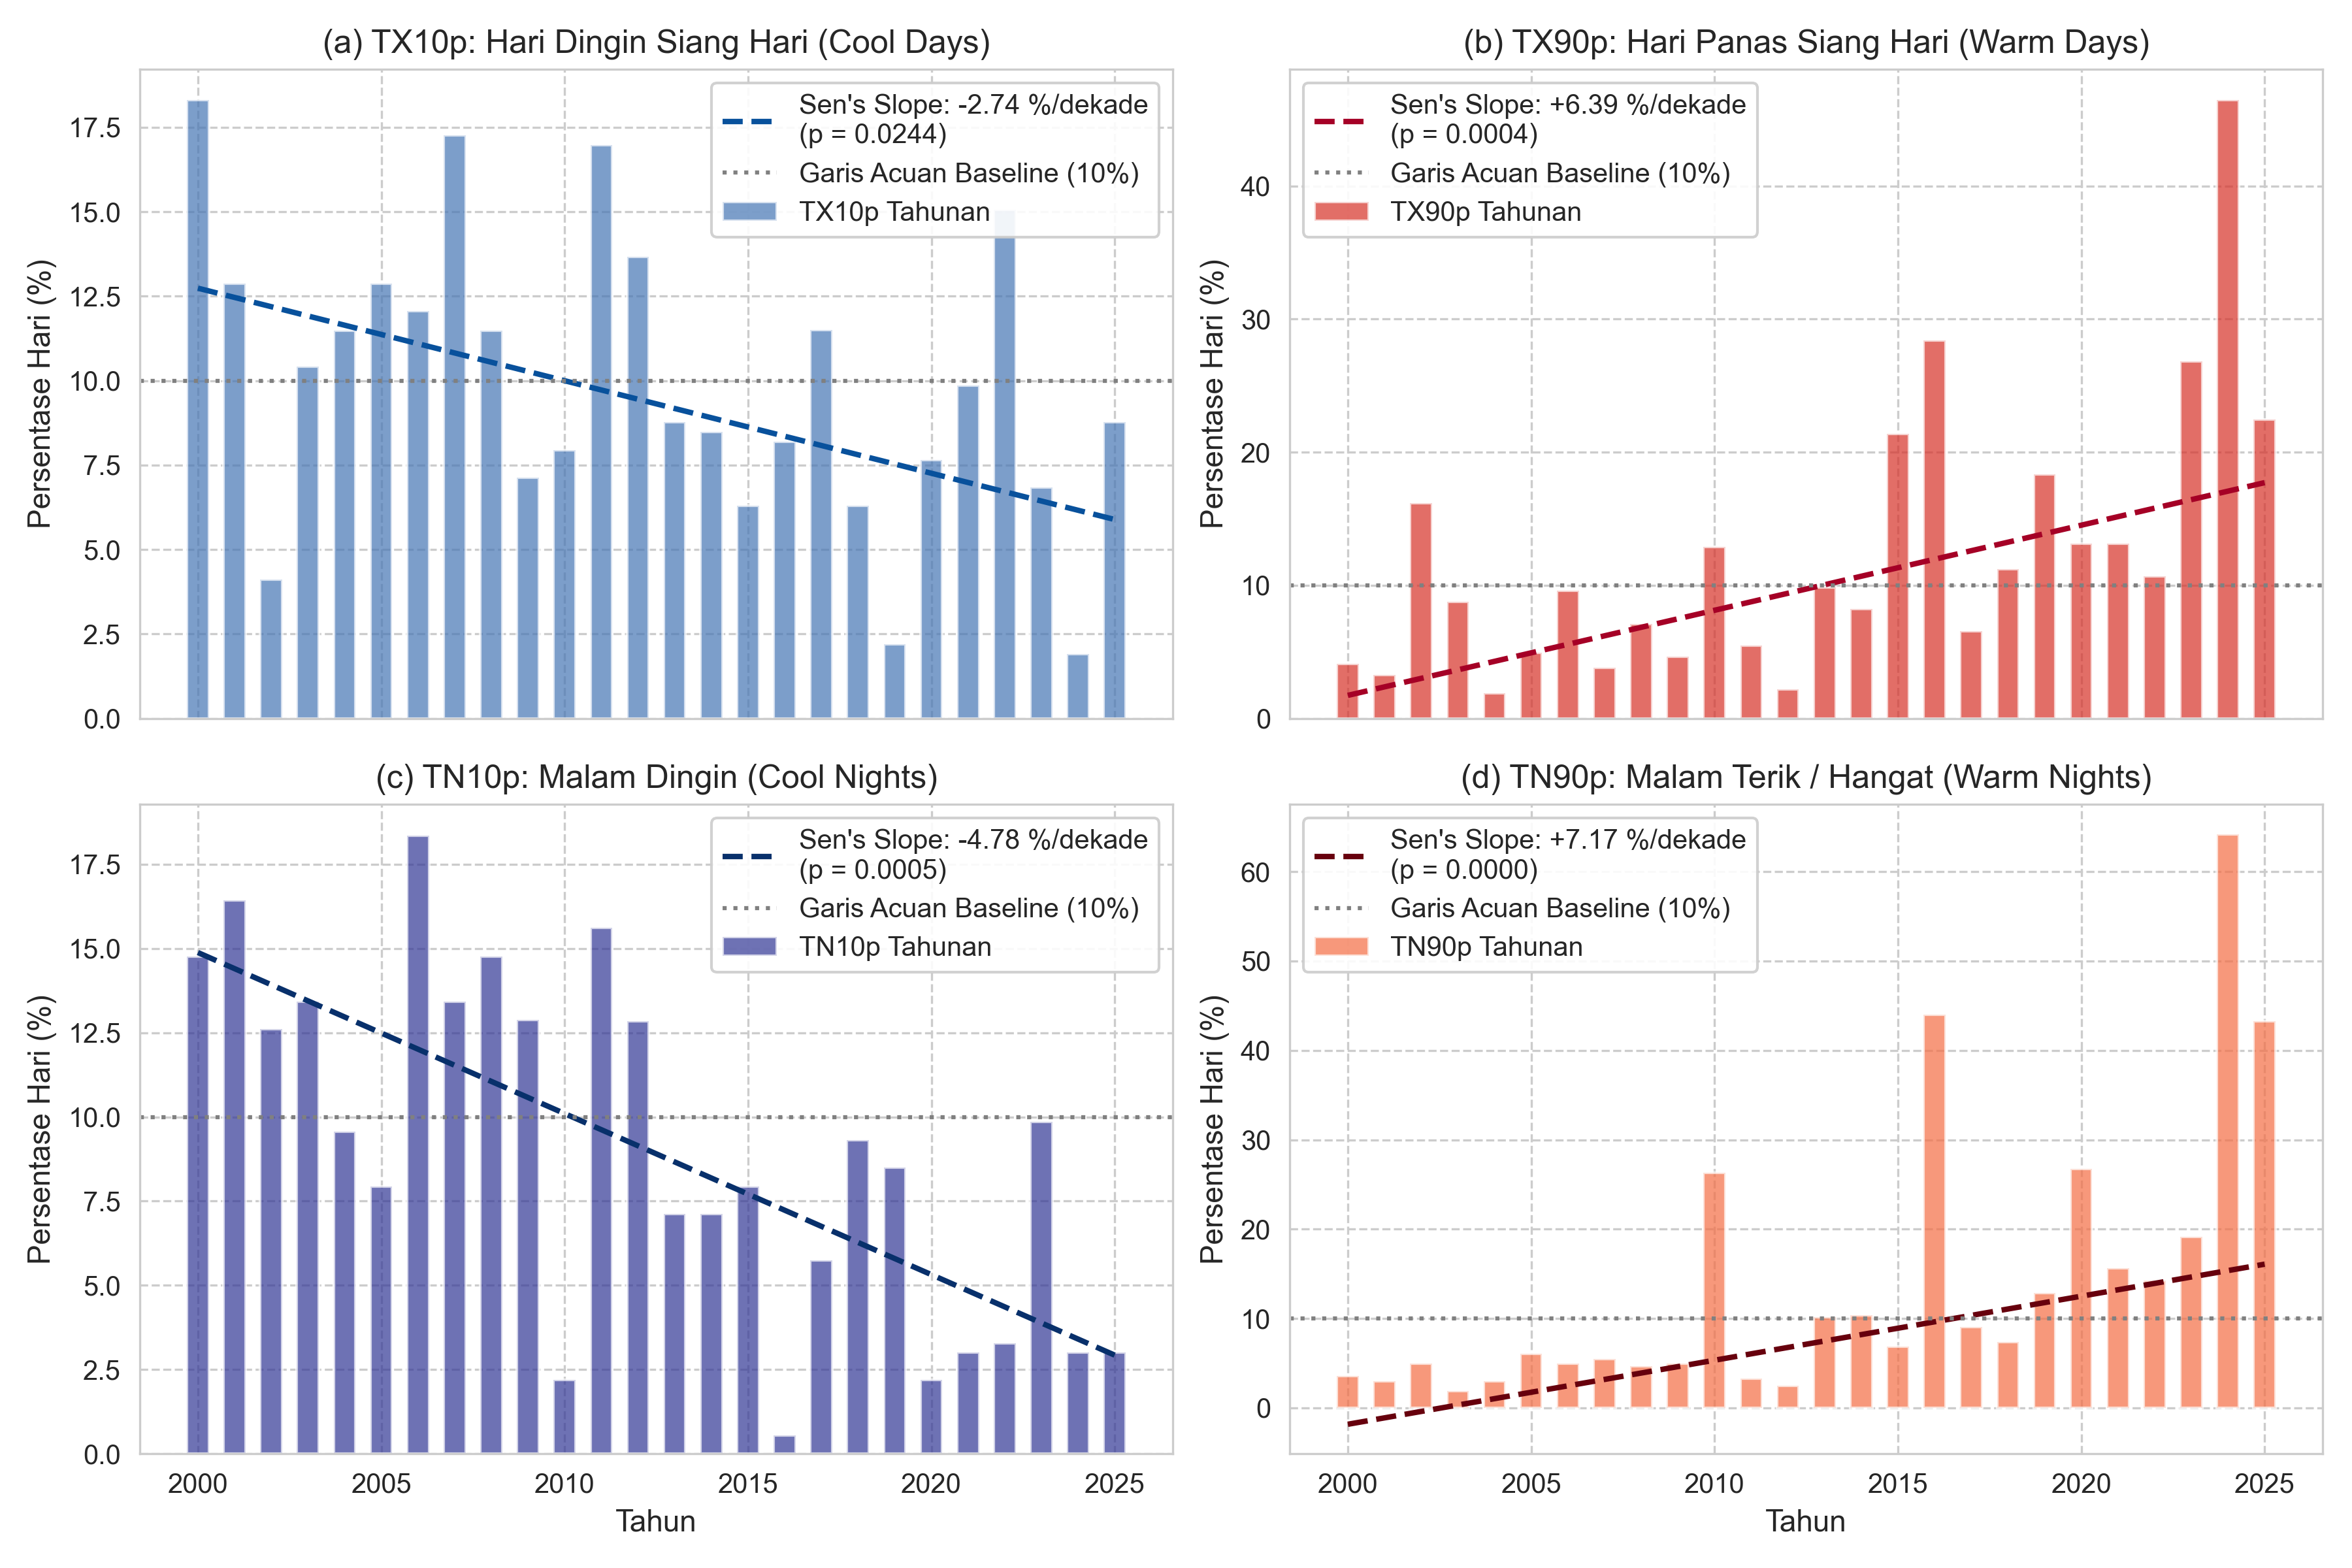
\includegraphics[width=\linewidth]{fig2_temperature_percentiles.png}
  \caption{Tren tahunan indeks suhu berbasis persentil (TX10p, TX90p, TN10p, TN90p) di Kabupaten Kebumen (2000--2025).}
  \label{fig:temp_percentiles}
\end{figure}

\subsubsection{Durasi Gelombang Panas/Dingin dan DTR}

Gambar~\ref{fig:spells_dtr} menampilkan WSDI, CSDI, dan DTR.

\textbf{WSDI} memiliki variabilitas antar-tahun yang sangat tinggi (Std = 16,6 hari). Nilai tertinggi terjadi pada 2015, 2023, dan 2024 (masing-masing 35, 58, dan 58 hari)---bertepatan dengan periode El Ni\~{n}o kuat.

\textbf{CSDI} menunjukkan tren turun signifikan ($Z_{MK} = -2{,}19$, $p = 0{,}028$, *), mengkonfirmasi berkurangnya periode suhu dingin. Indeks \textbf{FD} dan \textbf{ID} bernilai nol sepanjang periode, konsisten dengan iklim tropis Kebumen.

\begin{figure}[H]
  \centering
  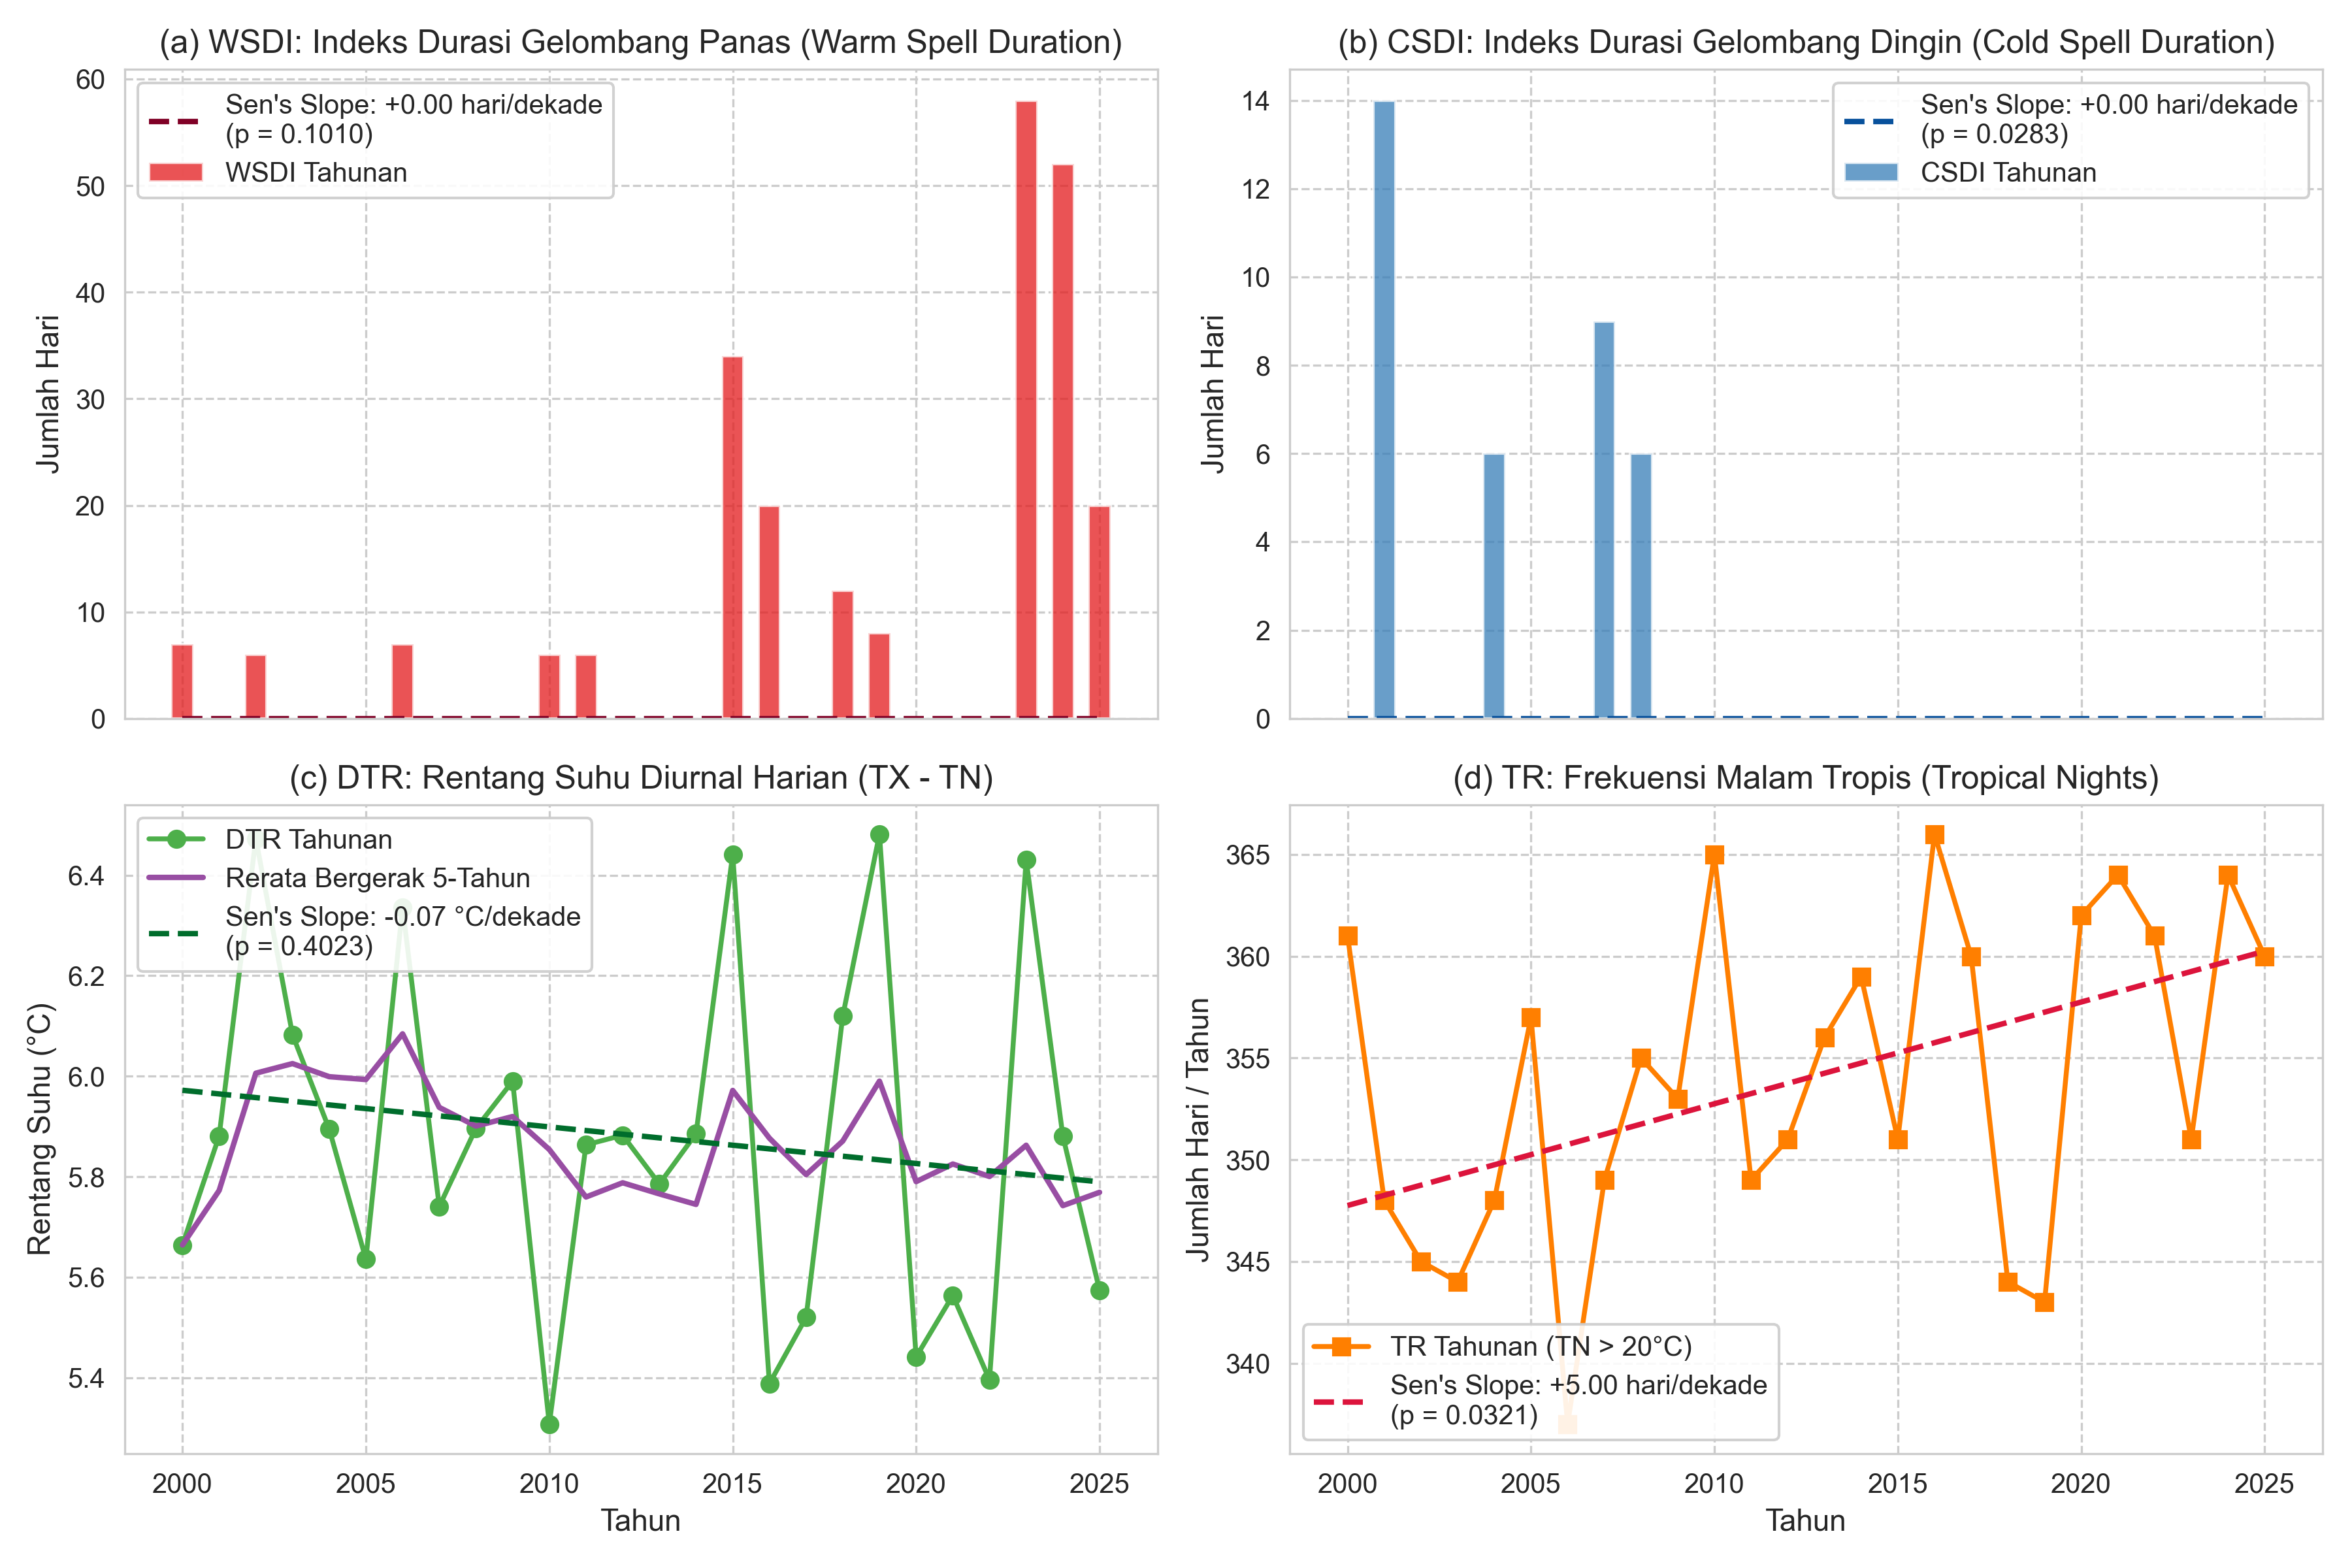
\includegraphics[width=\linewidth]{fig3_spells_and_dtr.png}
  \caption{Tren tahunan WSDI, CSDI, dan DTR di Kabupaten Kebumen (2000--2025).}
  \label{fig:spells_dtr}
\end{figure}

\subsection{Indeks Presipitasi: Tren dan Variabilitas}

\subsubsection{Presipitasi Maksimum (Rx1day, Rx5day)}

Gambar~\ref{fig:prec_maxima} menampilkan tren Rx1day dan Rx5day. Rata-rata curah hujan maksimum harian mencapai 116 mm dengan variabilitas tinggi (Std = 57 mm). Nilai ekstrem tertinggi terjadi pada 2003 (278,96 mm). Meski tren Sen's Slope menunjukkan +13,98 mm/dekade, uji \mk{} tidak menemukan signifikansi statistik.

\begin{figure}[H]
  \centering
  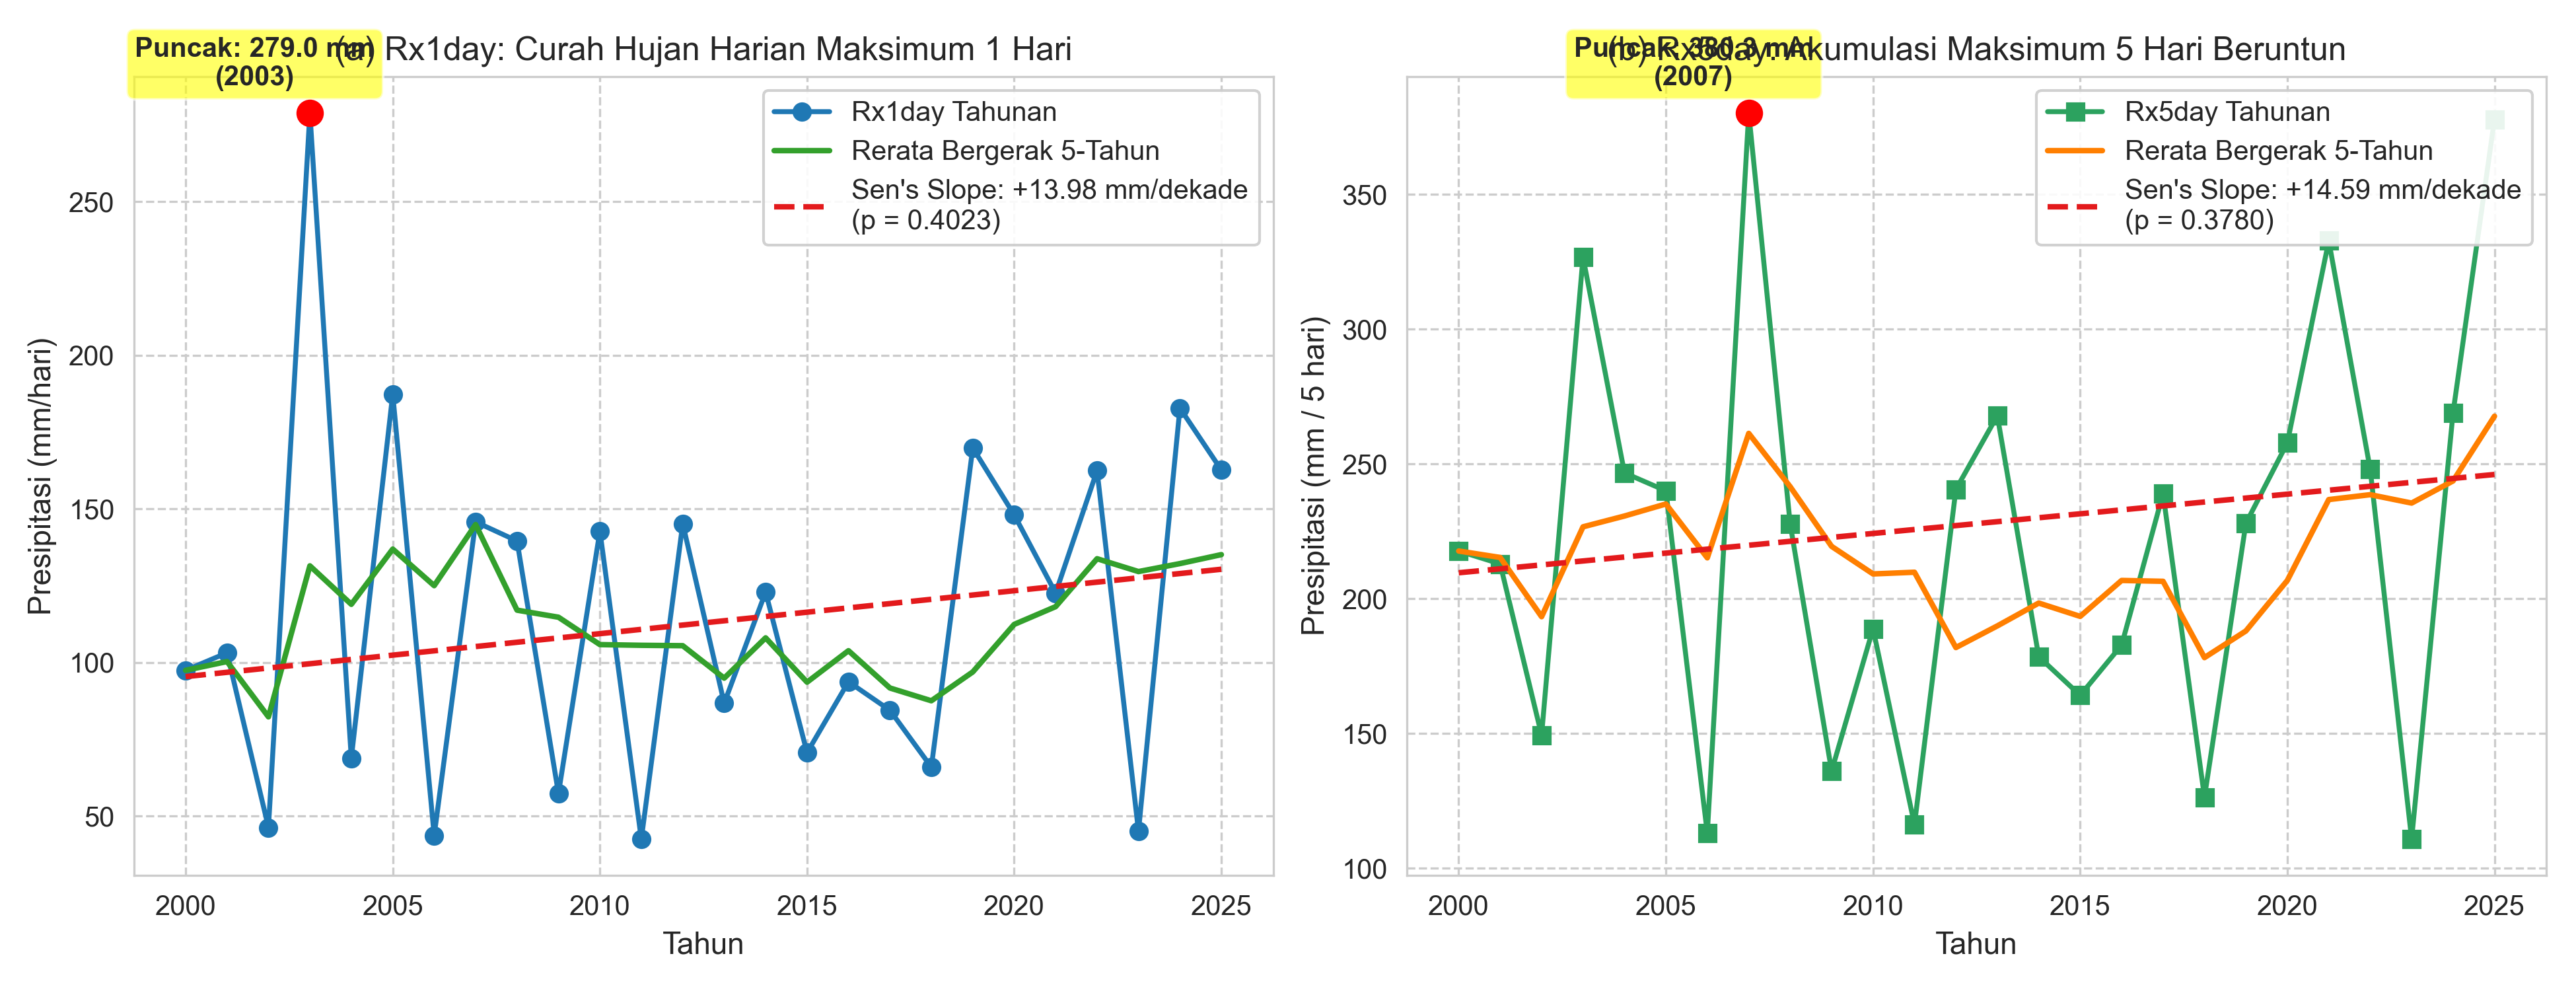
\includegraphics[width=\linewidth]{fig4_precipitation_maxima.png}
  \caption{Tren tahunan Rx1day dan Rx5day di Kabupaten Kebumen (2000--2025).}
  \label{fig:prec_maxima}
\end{figure}

\subsubsection{Total dan Intensitas Presipitasi (PRCPTOT, SDII)}

Gambar~\ref{fig:prec_totals} menunjukkan PRCPTOT dan SDII. Total curah hujan tahunan bervariasi dari 1.618 mm (2023) hingga 3.871 mm (2016) dengan rata-rata 2.734 mm/tahun. Tahun 2016 merupakan tahun terbasah (La Ni\~{n}a), sedangkan 2023 adalah tahun terkering (El Ni\~{n}o kuat).

\begin{figure}[H]
  \centering
  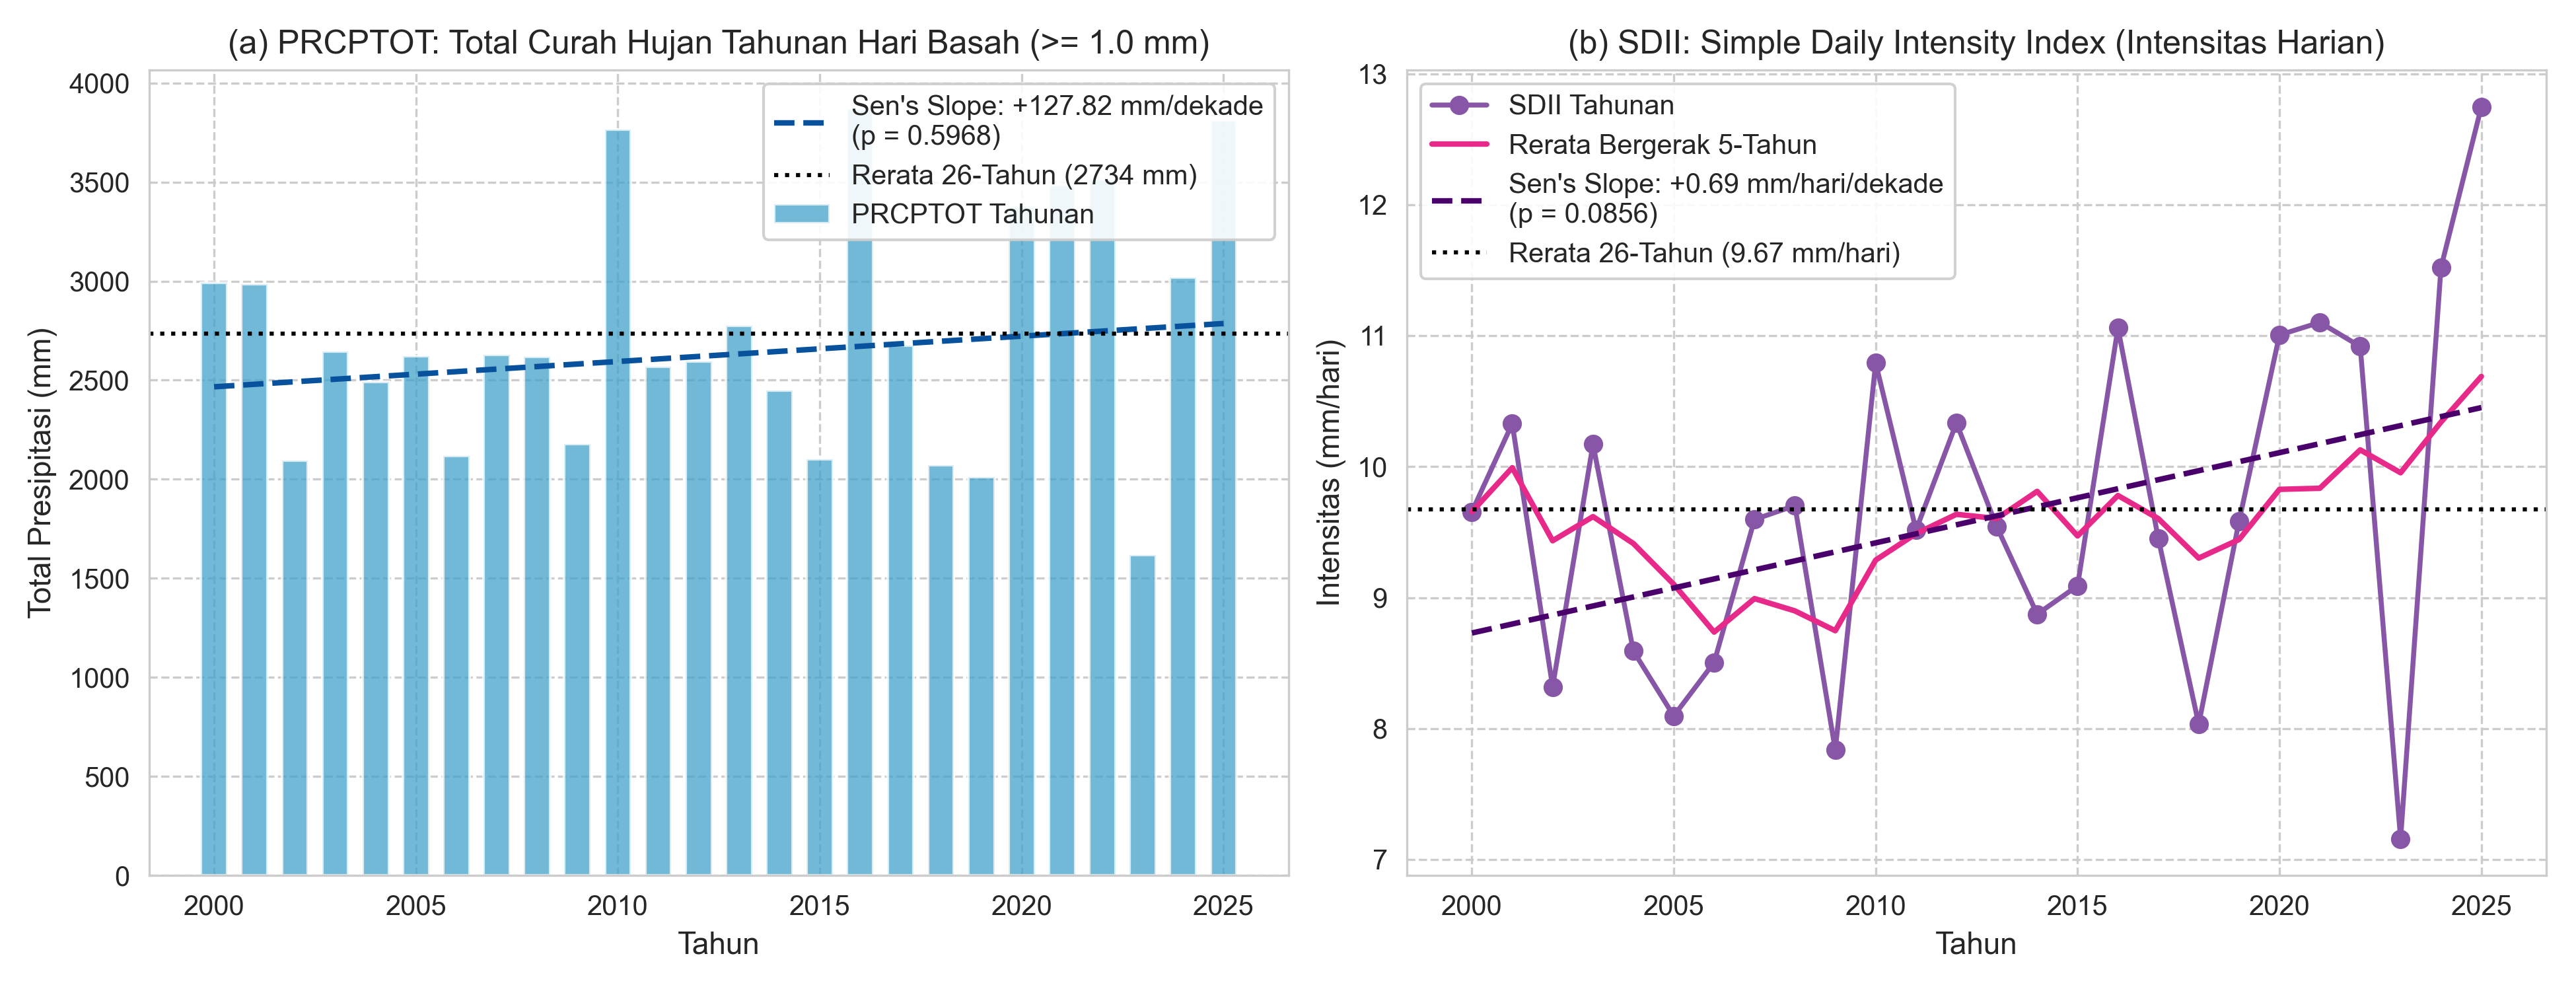
\includegraphics[width=\linewidth]{fig5_precipitation_totals_and_intensity.png}
  \caption{Tren PRCPTOT dan SDII di Kabupaten Kebumen (2000--2025).}
  \label{fig:prec_totals}
\end{figure}

\subsubsection{Hari Hujan Lebat (R10mm, R20mm, Rnnmm)}

Gambar~\ref{fig:extreme_days} menampilkan frekuensi hari hujan berbasis ambang batas. Rata-rata terdapat 92 hari/tahun dengan curah hujan $\geq$10 mm, 30 hari dengan $\geq$20 mm, dan 3,6 hari dengan $\geq$50 mm.

\begin{figure}[H]
  \centering
  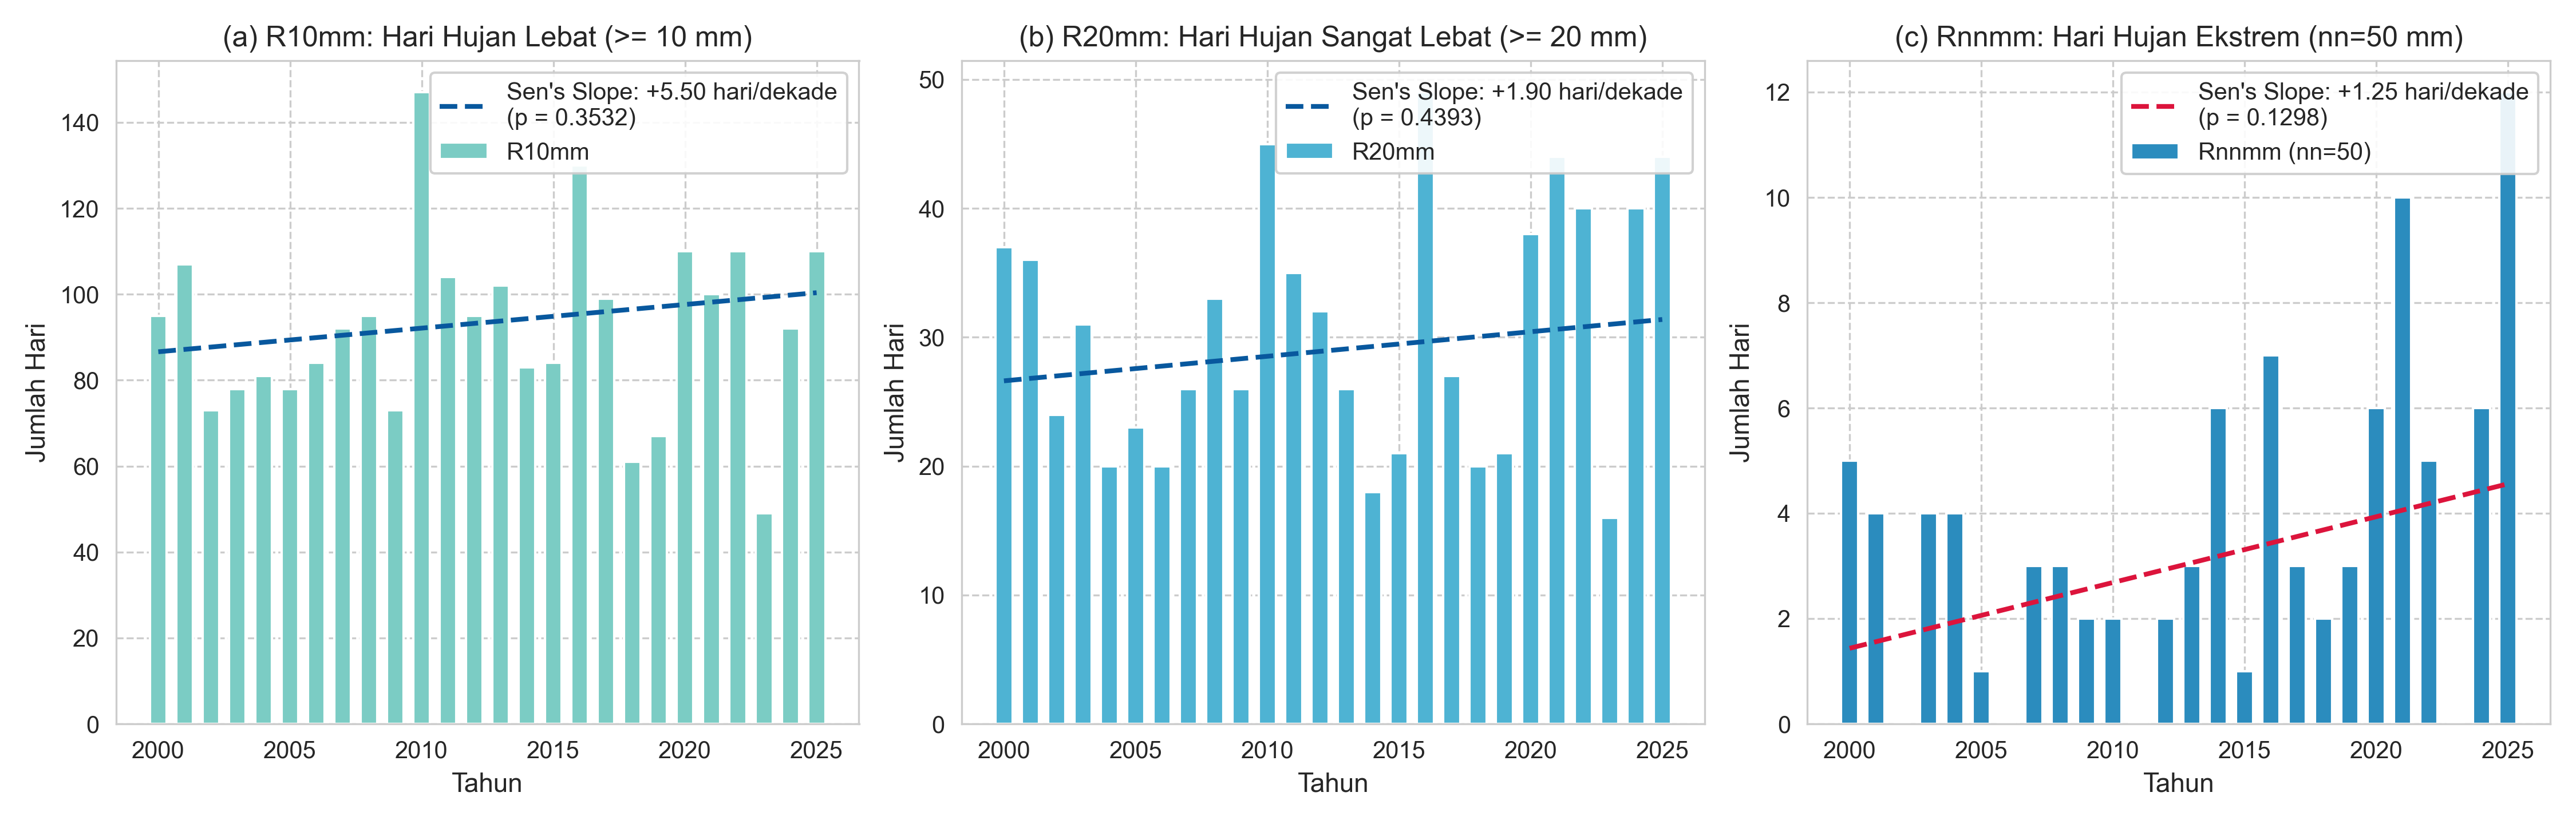
\includegraphics[width=\linewidth]{fig6_extreme_precipitation_days.png}
  \caption{Frekuensi tahunan R10mm, R20mm, dan Rnnmm ($nn=50$ mm) di Kabupaten Kebumen (2000--2025).}
  \label{fig:extreme_days}
\end{figure}

\subsubsection{Hari Kering dan Basah Berurutan (CDD, CWD)}

Gambar~\ref{fig:spells_prec} menunjukkan CDD dan CWD. Penurunan \textbf{CWD} adalah temuan yang paling signifikan secara presipitasi: $Z_{MK} = -2{,}30$ ($p = 0{,}022$, *) dengan laju $-$10,77 hari/dekade. Pada 2000, CWD mencapai 119 hari, namun tren jangka panjang menunjukkan pengurangan durasi musim hujan yang berkelanjutan---berimplikasi pada ketersediaan air bagi pertanian tadah hujan.

\begin{figure}[H]
  \centering
  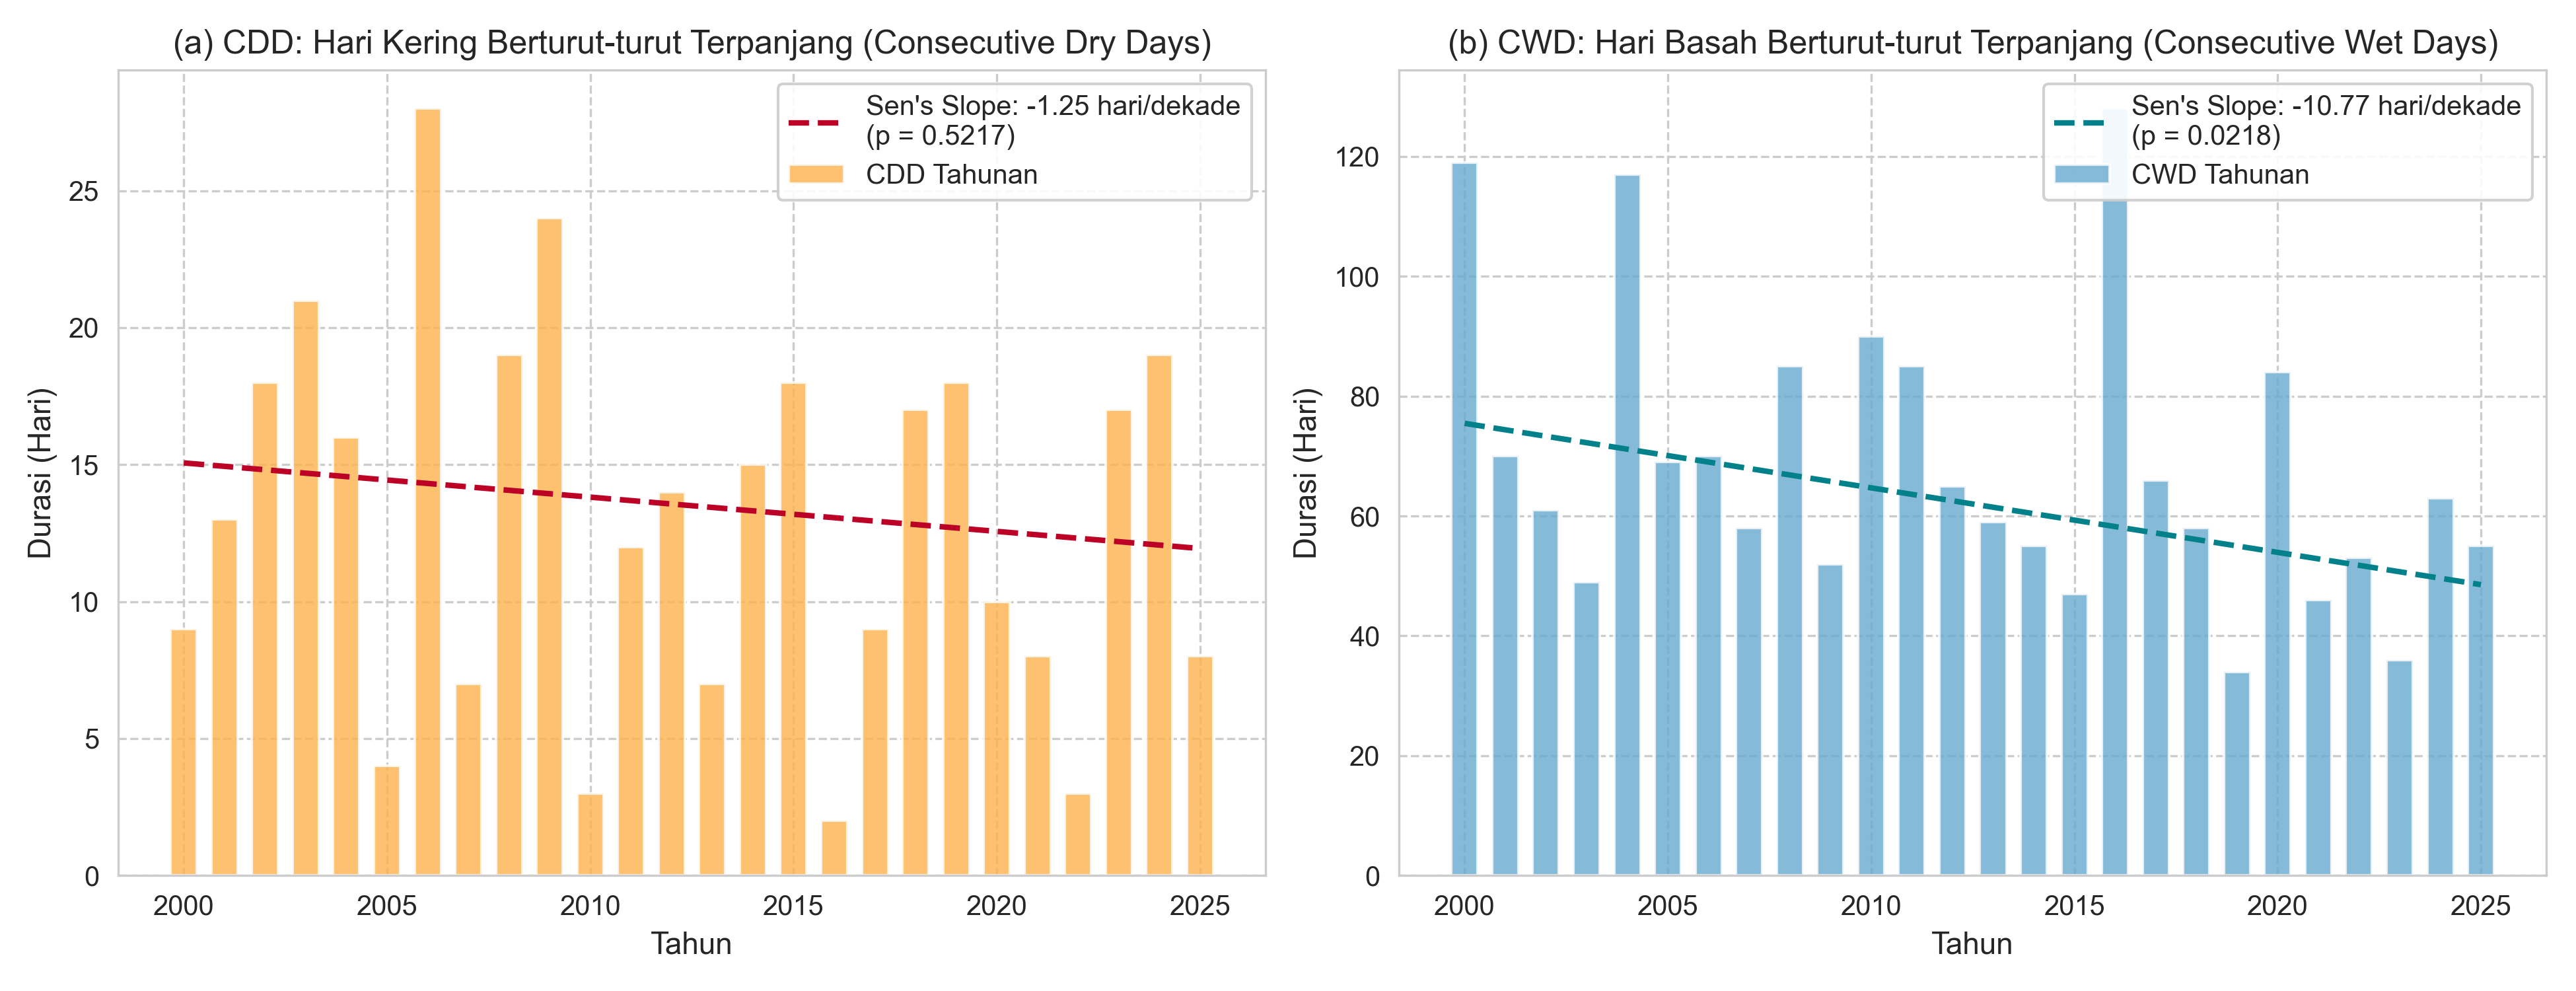
\includegraphics[width=\linewidth]{fig7_dry_wet_spells.png}
  \caption{Tren CDD dan CWD di Kabupaten Kebumen (2000--2025). Penurunan CWD signifikan secara statistik ($p = 0{,}022$).}
  \label{fig:spells_prec}
\end{figure}

\subsection{Perbandingan Antarproduct Satelit}

Gambar~\ref{fig:satellite_comparison} menampilkan perbandingan indeks presipitasi dari keempat produk satelit. Tabel~\ref{tab:sat_climatology} merangkum rata-rata klimatologis.

\begin{table}[H]
  \centering
  \caption{Perbandingan rata-rata klimatologis (2000--2025) indeks presipitasi dari empat produk satelit.}\label{tab:sat_climatology}
  \small
  \begin{tabular}{lrrrrrrrrrrr}
    \toprule
    \textbf{Produk} & \textbf{Rx1} & \textbf{Rx5} & \textbf{SDII} & \textbf{PRCP} & \textbf{R10} & \textbf{R20} & \textbf{Rnn} & \textbf{R95p} & \textbf{R99p} & \textbf{CDD} & \textbf{CWD} \\
    \midrule
    CHIRPS & 62,96 & 165,19 & 10,25 & 2.676 & 95,85 & 35,58 & 2,23 & 562 & 168 & 25 & 62 \\
    ERA5   & 104,47 & 220,94 & 9,26 & 2.554 & 81,42 & 28,00 & 3,62 & 723 & 293 & 14 & 57 \\
    GSMaP  & 90,39 & 178,81 & 13,59 & 2.516 & 84,88 & 41,38 & 5,08 & 523 & 167 & 43 & 19 \\
    IMERG  & 129,28 & 251,93 & 16,14 & 3.063 & 90,38 & 50,31 & 11,38 & 714 & 228 & 39 & 26 \\
    \bottomrule
  \end{tabular}
\end{table}

\begin{figure}[H]
  \centering
  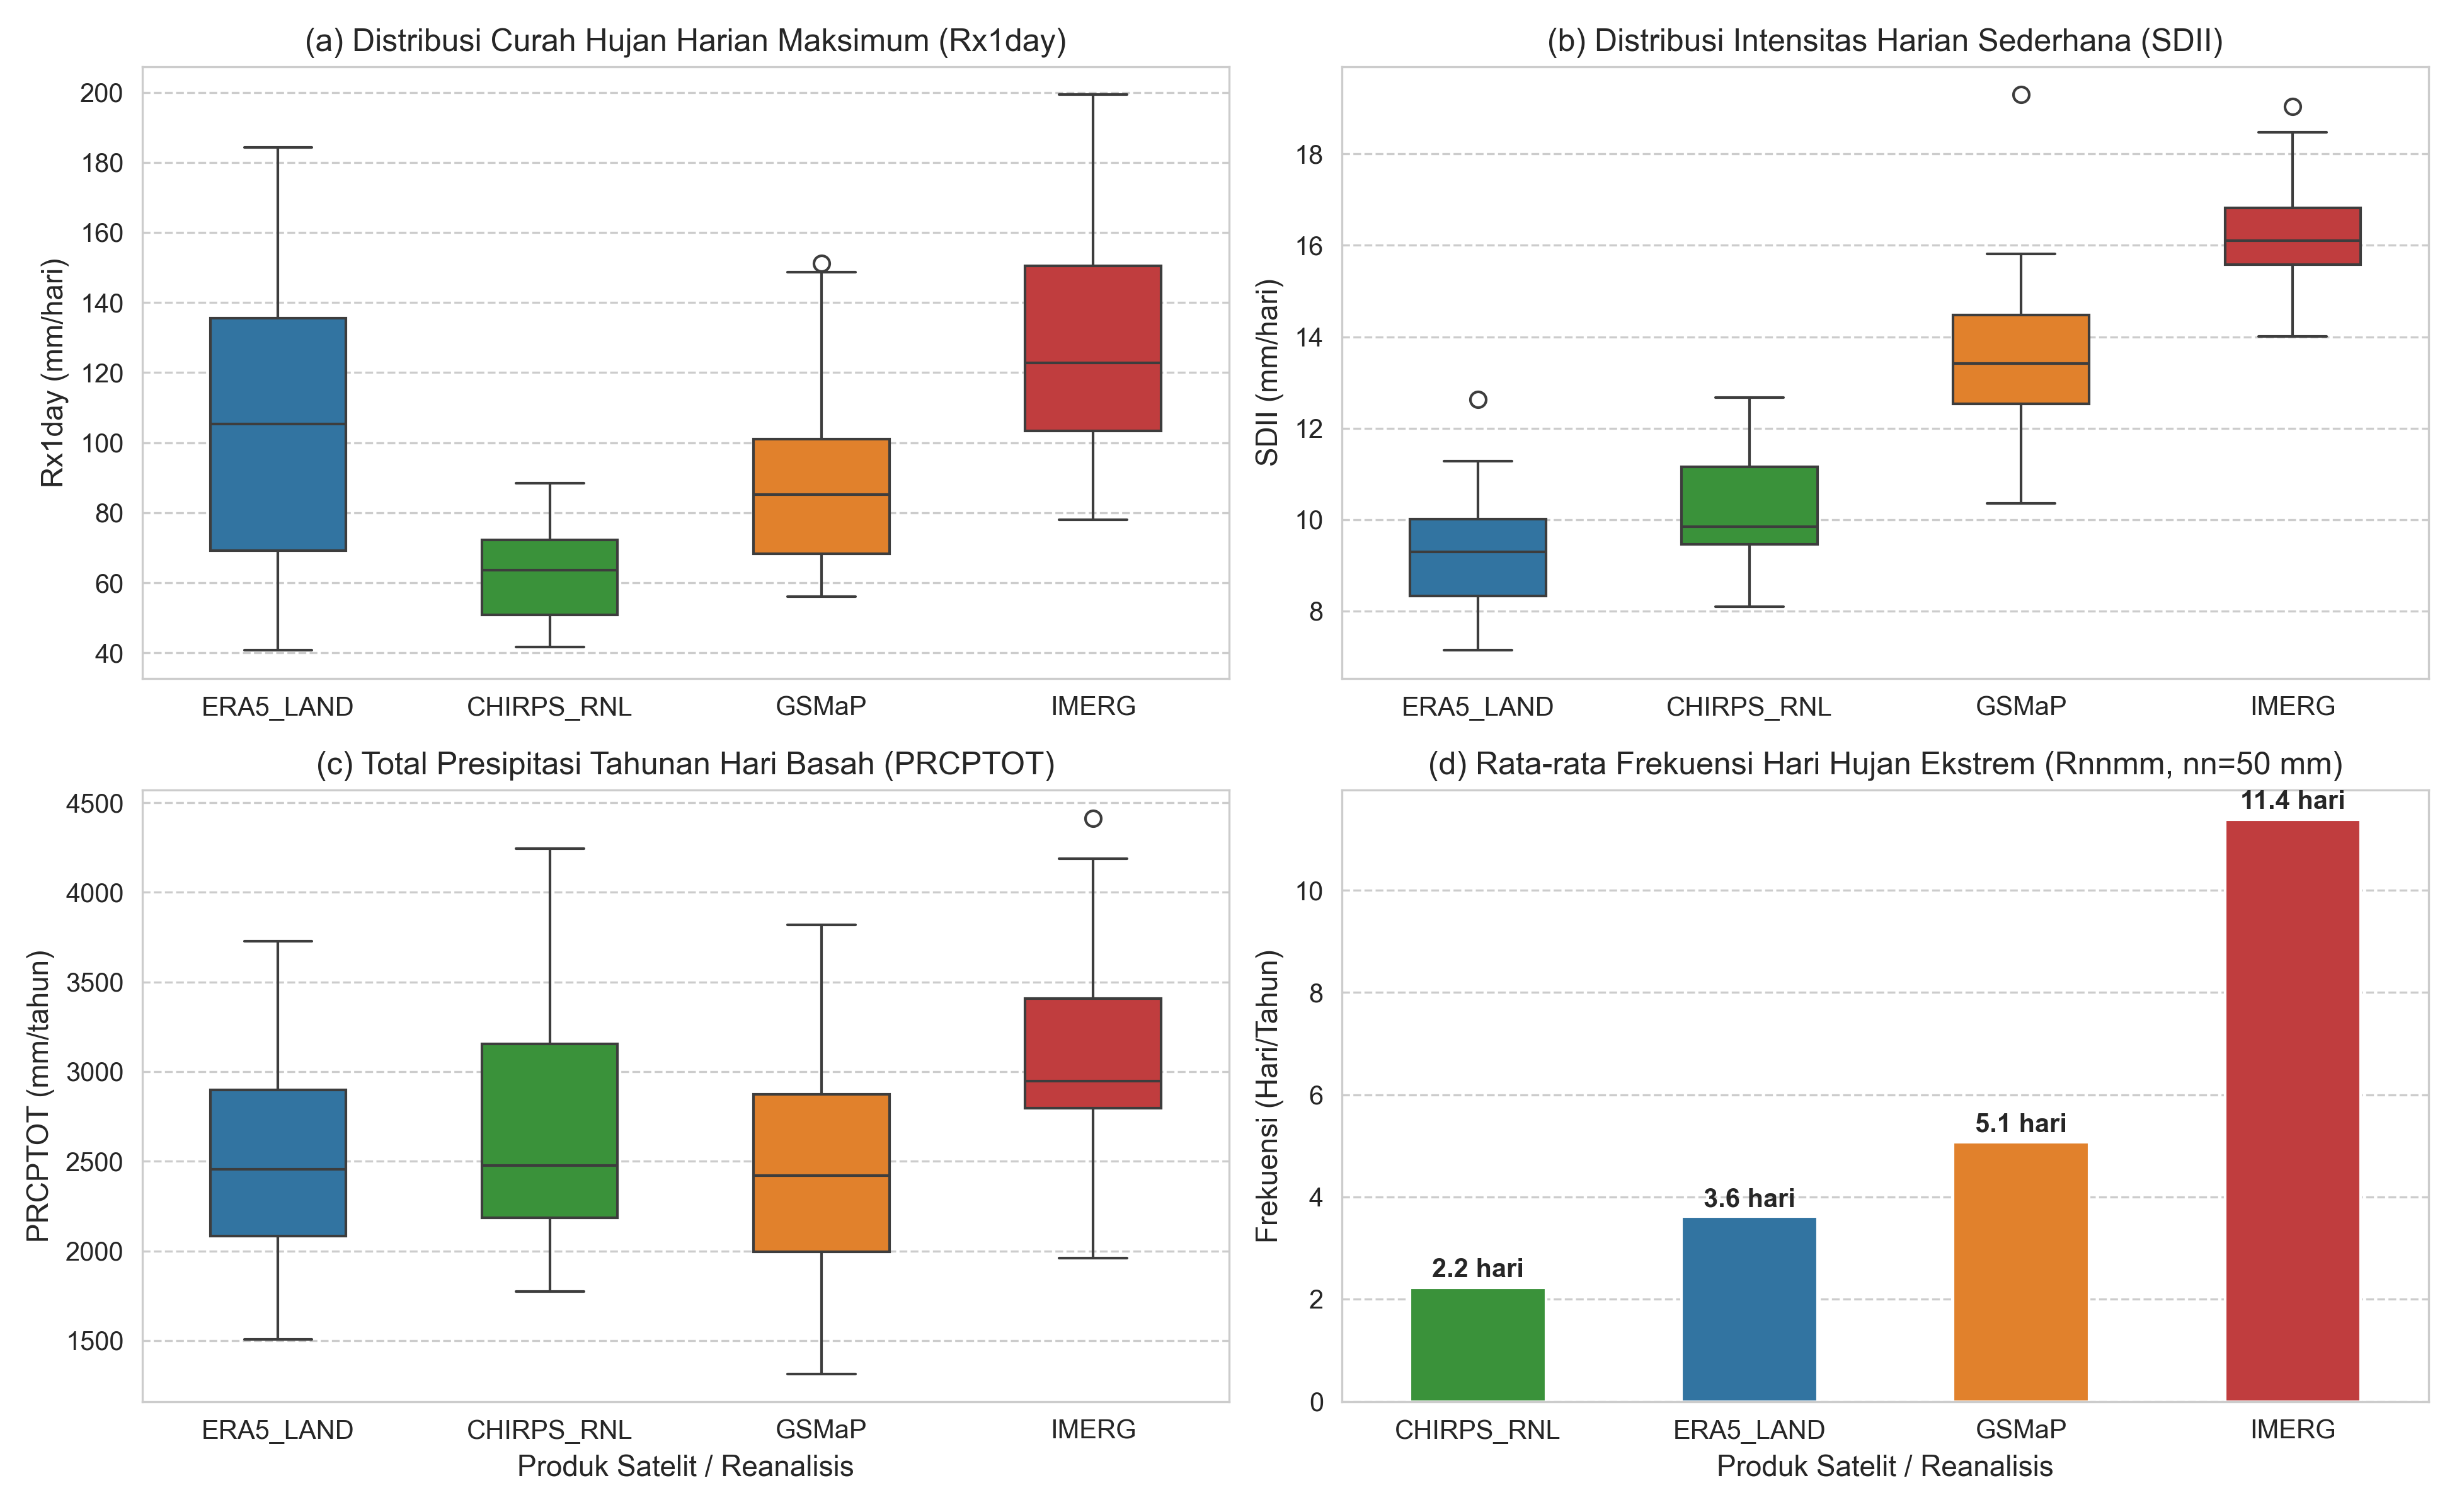
\includegraphics[width=\linewidth]{fig8_satellite_intercomparison_radar_corr.png}
  \caption{Perbandingan radar (kiri) dan matriks korelasi (kanan) indeks presipitasi dari empat produk satelit di Kabupaten Kebumen.}
  \label{fig:satellite_comparison}
\end{figure}

\textbf{IMERG} secara konsisten menghasilkan estimasi presipitasi tertinggi untuk Rx1day (129 mm), SDII (16,14 mm/hari), dan PRCPTOT (3.063 mm). Sebaliknya, \textbf{CHIRPS\_RNL} memberikan estimasi konservatif untuk Rx1day (63 mm). Nilai \textbf{CDD} dari GSMaP (43 hari) dan IMERG (39 hari) jauh lebih tinggi dibandingkan ERA5-Land (14 hari), mengindikasikan bahwa produk satelit cenderung meremehkan curah hujan ringan di bawah ambang batas 1 mm.

\subsection{Matriks Korelasi Antar-Indeks ETCCDI}

Gambar~\ref{fig:correlation_matrix} menampilkan matriks korelasi Spearman untuk 23 indeks \etccdi{} yang memiliki variasi antar-tahun; FD, ID, SU, dan GSL yang konstan atau hampir konstan tidak ditampilkan agar matriks tetap informatif.

\begin{figure}[H]
  \centering
  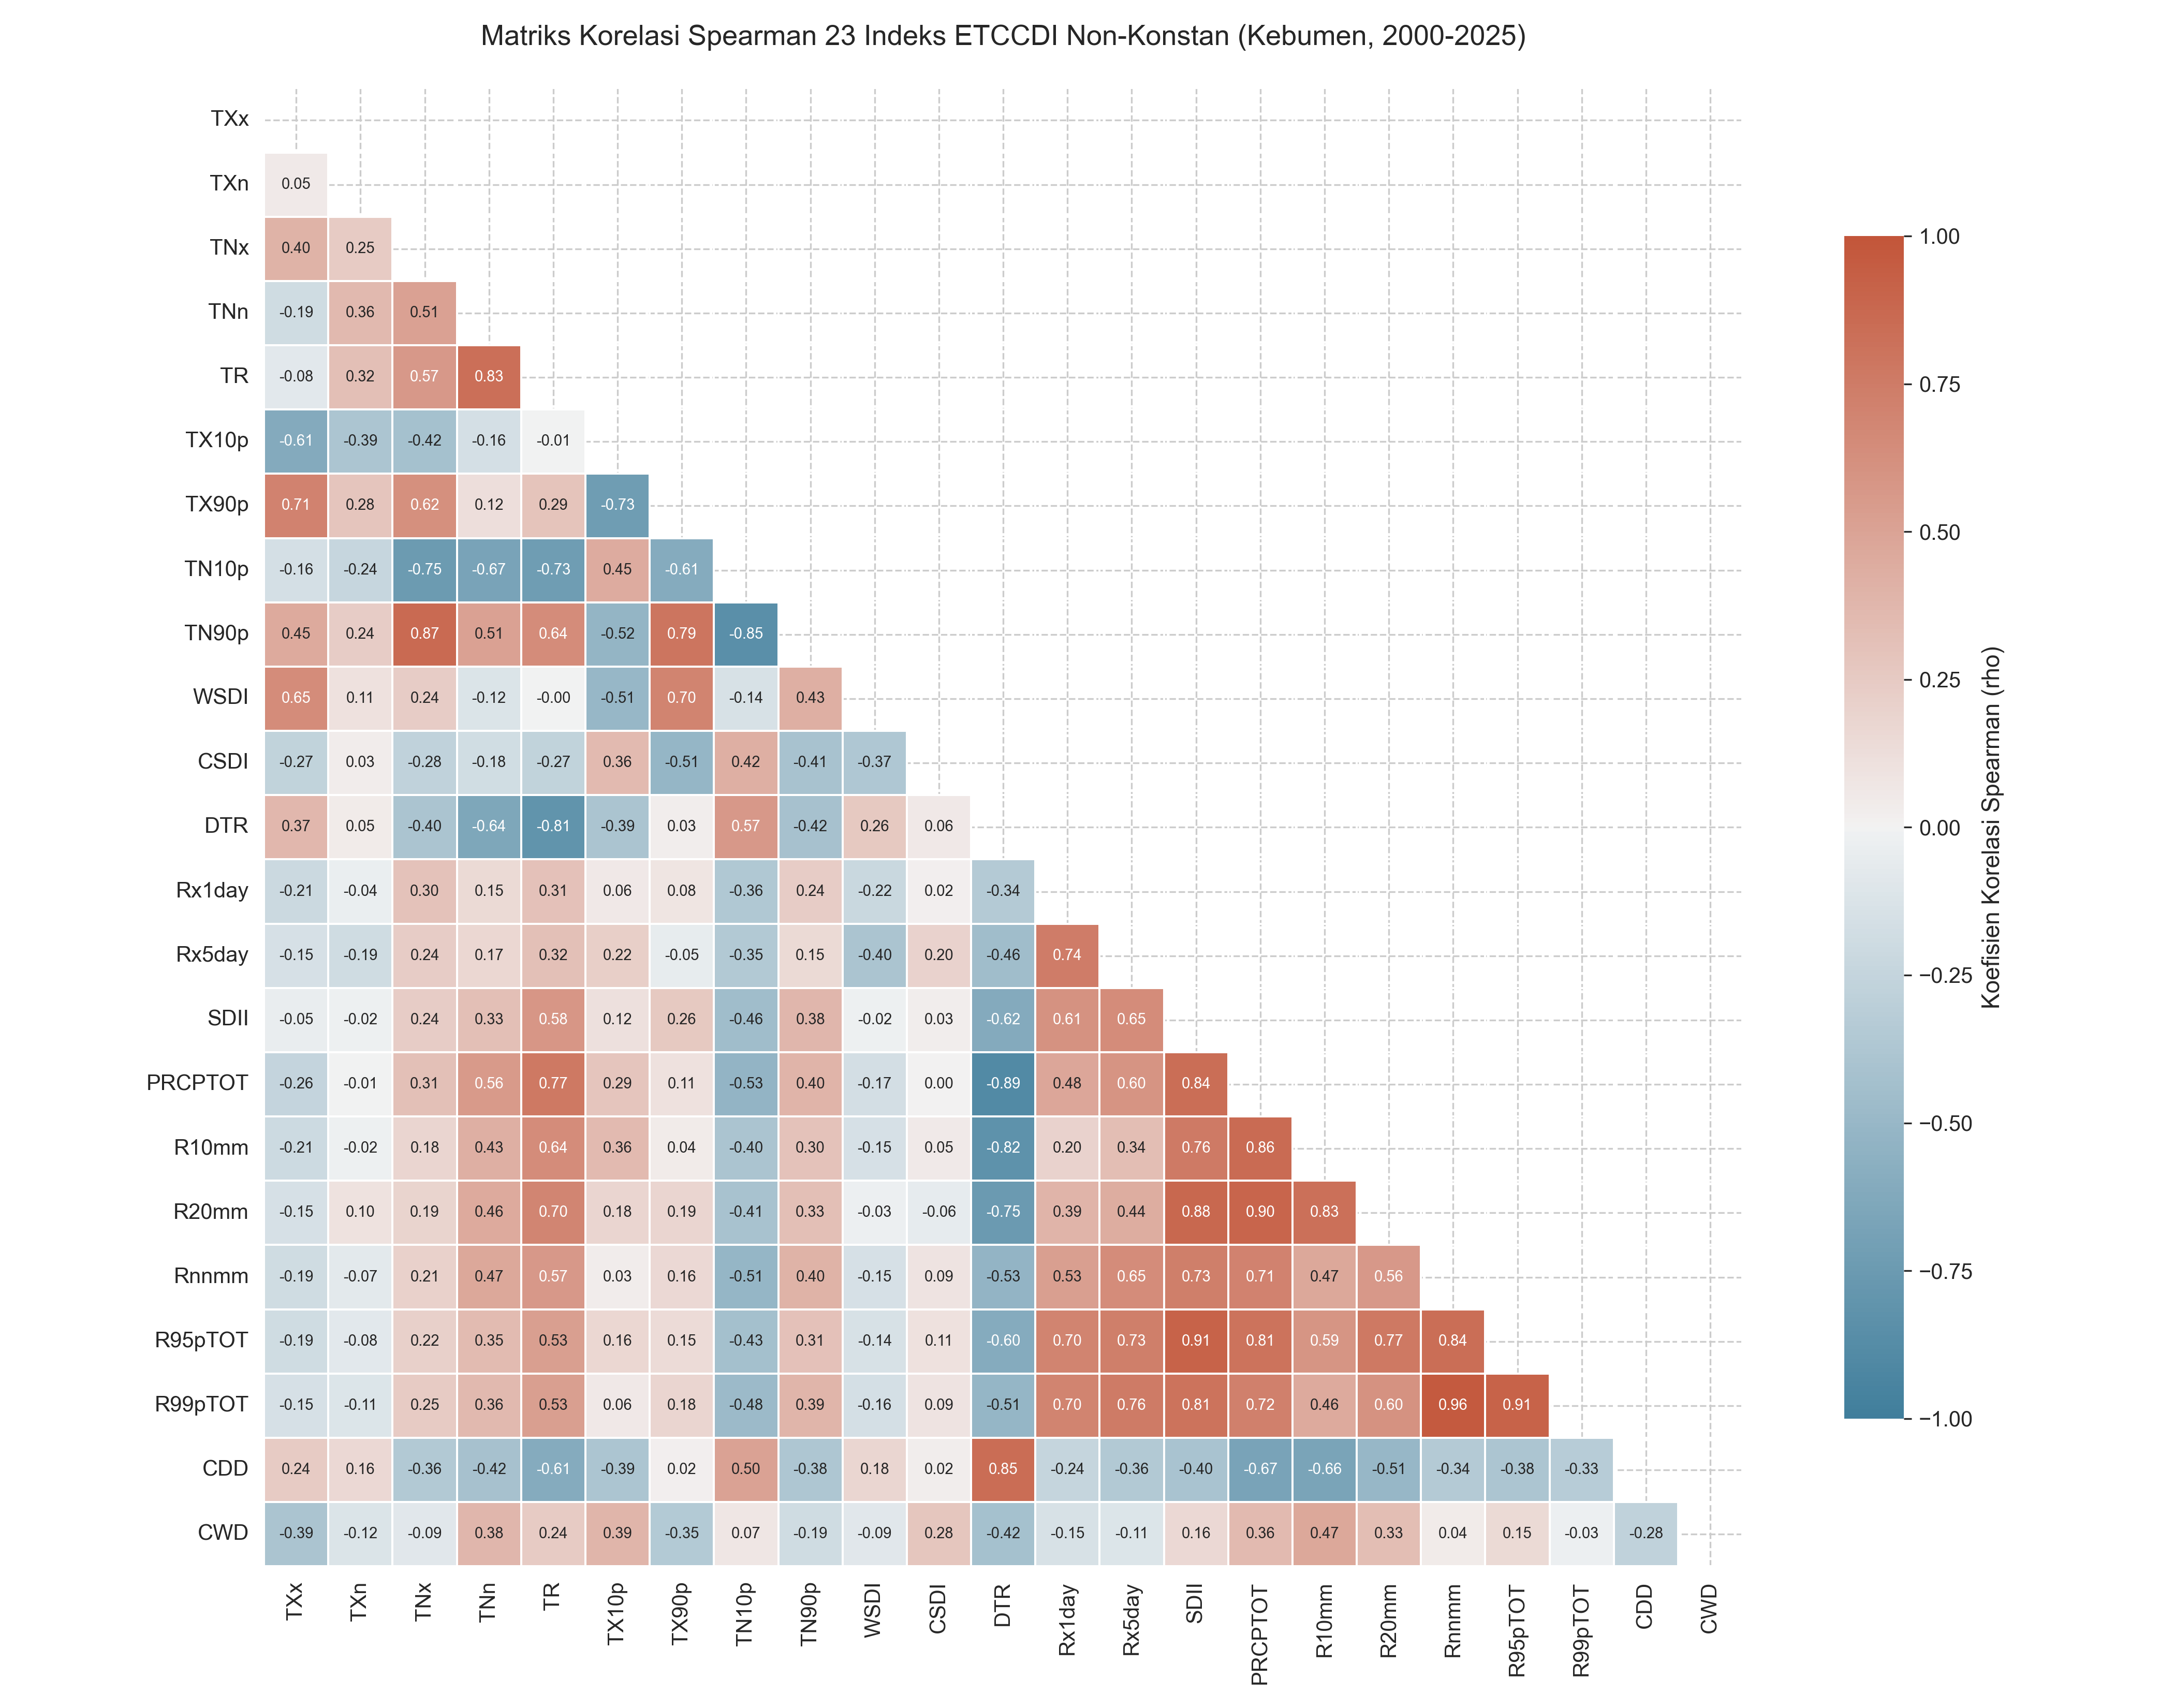
\includegraphics[width=\linewidth]{fig9_etccdi_correlation_matrix.png}
  \caption{Matriks korelasi Spearman 23 indeks ETCCDI non-konstan di Kebumen (2000--2025). Merah: korelasi positif kuat; Biru: korelasi negatif kuat.}
  \label{fig:correlation_matrix}
\end{figure}

Korelasi antar-indeks yang menonjol:
\begin{itemize}
  \item \textbf{TN90p--TX90p} ($r \approx +0{,}82$): episode panas mempengaruhi seluruh siklus diurnal.
  \item \textbf{PRCPTOT--R10mm--R20mm} ($r > +0{,}85$): variabilitas curah hujan tahunan didominasi kejadian lebat.
  \item \textbf{CWD--PRCPTOT} ($r \approx +0{,}74$): musim hujan lebih panjang berkorelasi dengan total hujan lebih tinggi.
  \item \textbf{TN90p--WSDI} ($r \approx +0{,}76$): tahun dengan banyak malam hangat juga lebih sering mengalami gelombang panas siang.
\end{itemize}

%% 5. DISKUSI
\section{Diskusi}

\subsection{Sinyal Pemanasan: Dominasi Suhu Minimum}

Hasil analisis mengkonfirmasi pemanasan signifikan di Kebumen selama 2000--2025, dengan sinyal terkuat pada suhu minimum malam hari. Laju pemanasan TNx (+0,37\degC{}/dekade) lebih tinggi dibandingkan TXx ($\approx$+0,27\degC{}/dekade), konsisten dengan fenomena \textit{warming asymmetry} di Asia Tenggara. Peningkatan kelembaban atmosfer dan tutupan awan rendah pada malam hari menahan radiasi inframerah (\textit{greenhouse trapping}), yang diperkuat oleh uap air dari Samudera Hindia di wilayah pesisir Kebumen.

\subsection{Penurunan Durasi Musim Hujan: Implikasi bagi Pertanian}

Penurunan signifikan CWD ($-$10,77 hari/dekade) meski total curah hujan tidak berubah signifikan mengimplikasikan kompres durasi hujan ke periode lebih pendek---konsisten dengan tren SDII naik. Bagi sektor pertanian padi di Kebumen yang bergantung pada irigasi tadah hujan, perubahan ini berpotensi mempengaruhi pola tanam.

\subsection{Pengaruh ENSO}

Variabilitas PRCPTOT yang tinggi (Std = 609 mm) dan kisaran antara tahun terkering (2023: 1.618 mm) dan terbasah (2016: 3.871 mm) menunjukkan dominansi ENSO. Tahun-tahun El Ni\~{n}o kuat (2015, 2019, 2023) konsisten dengan PRCPTOT lebih rendah dan TXx lebih tinggi. La Ni\~{n}a (2010, 2016, 2020--2022) berkaitan dengan PRCPTOT lebih tinggi dan CWD lebih panjang.

\subsection{Ketidakpastian Data Satelit}

Rentang Rx1day antar-produk yang lebar (63 mm CHIRPS vs 129 mm IMERG) menegaskan perlunya validasi dengan data \textit{in-situ}. IMERG yang menggunakan sensor radar aktif (GPM-DPR) umumnya lebih akurat untuk kejadian ekstrem, sedangkan CHIRPS yang menggabungkan data stasiun lebih representatif untuk rata-rata curah hujan.

%% 6. KESIMPULAN
\section{Kesimpulan}

Penelitian ini berhasil menganalisis 27 indeks iklim ekstrem \etccdi{} di Kabupaten Kebumen selama 26 tahun (2000--2025). Kesimpulan utama:

\begin{enumerate}
  \item \textbf{Pemanasan Nyata pada Suhu Minimum Malam Hari:}
    TN90p meningkat $+7{,}17\%$/dekade; TN10p menurun $-4{,}78\%$/dekade; TNx meningkat $+0{,}37$\degC{}/dekade (semua $p < 0{,}001$).
  \item \textbf{Pemanasan Siang Hari juga Signifikan:}
    TX90p meningkat $+6{,}39\%$/dekade; TX10p menurun $-2{,}74\%$/dekade; TR meningkat $+5{,}0$ hari/dekade.
  \item \textbf{Tidak Ada Hari Beku dan Hari Es:}
    FD dan ID bernilai nol sepanjang 2000--2025, konsisten dengan iklim tropis.
  \item \textbf{Presipitasi: Penurunan CWD Signifikan:}
    CWD menurun $-10{,}77$ hari/dekade ($p = 0{,}022$). PRCPTOT rata-rata 2.734 mm/tahun dipengaruhi kuat oleh ENSO.
  \item \textbf{Ketidakpastian Antarproduct Satelit Besar:}
    Rentang Rx1day antar-produk mencapai 2$\times$ (CHIRPS vs IMERG). Validasi data \textit{in-situ} sangat direkomendasikan.
\end{enumerate}

Tanda-tanda perubahan iklim terdeteksi di Kabupaten Kebumen---terutama percepatan pemanasan malam hari dan perubahan pola musim hujan---yang memerlukan adaptasi dalam pengelolaan sumber daya air dan ketahanan pangan daerah.

%% UCAPAN TERIMA KASIH
\section*{Ucapan Terima Kasih}
\addcontentsline{toc}{section}{Ucapan Terima Kasih}

Penulis mengucapkan terima kasih kepada ECMWF atas penyediaan data ERA5-Land melalui \textit{Copernicus Climate Data Store}, kepada tim Google Earth Engine atas platform komputasi geospasial, serta kepada Stasiun AWS Jerukagung Kebumen atas data validasi lapangan. Penelitian ini merupakan bagian dari thesis S1 di Universitas Putra Bangsa.

%% DAFTAR PUSTAKA
\newpage
\bibliography{references}

\end{document}
